\section{Results and Discussion} \label{s:results}
This section will present the results of the work and discuss their significance. The piston valve is first compared to the previous results obtained with the rupture disks to ensure the valve works as intended and provides the desired pressurization. Then, the piston valve is compared to itself to determine the valve's repeatability and predictability. The valve is then tested for re-usability and durability.

\subsection{Rupture Disk Results}

\begin{figure}[tb]
    \vspace{16pt}
    \centering
    \begin{subfigure}[t]{0.45\textwidth}
        \centering
        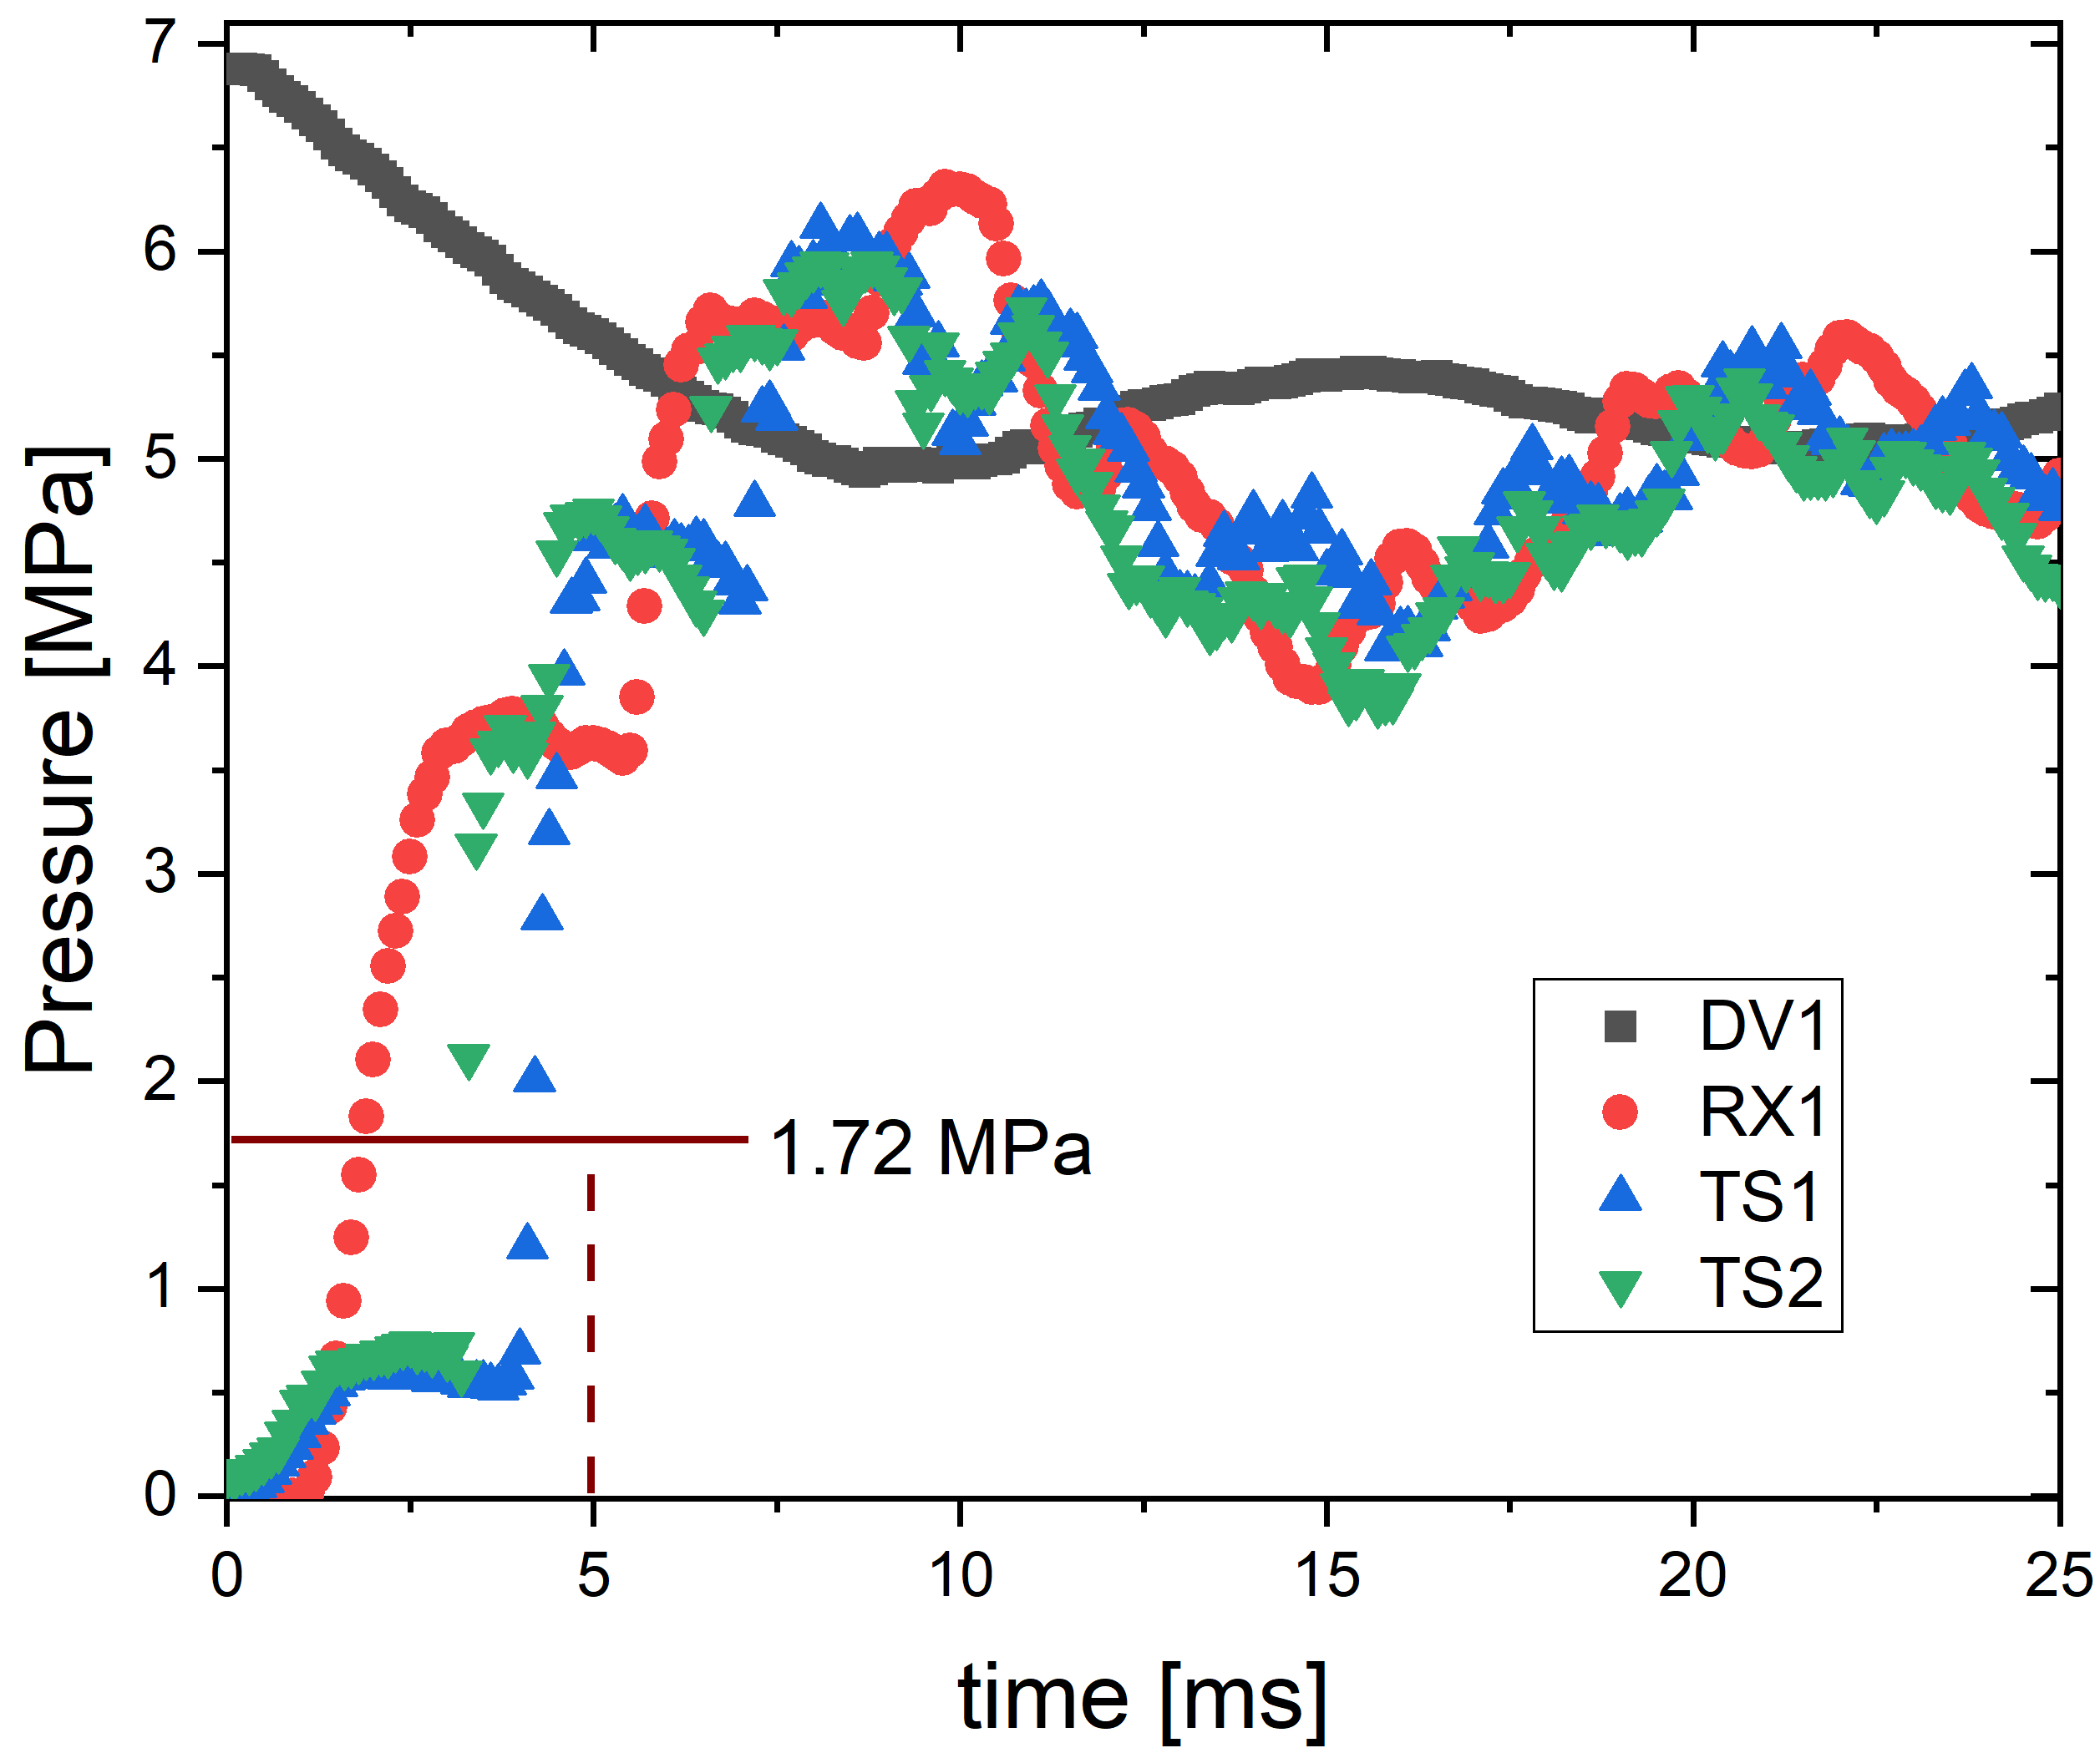
\includegraphics[width=0.9\textwidth]{results/plots/1000psi_MPa_BD_1inch.png}
        \caption{Pressure over time for rupture disk HENRI test in a cylindrical test section.}
        \label{fig:cyl disk}
    \end{subfigure}
    \hfill
    \begin{subfigure}[t]{0.45\textwidth}
        \centering
        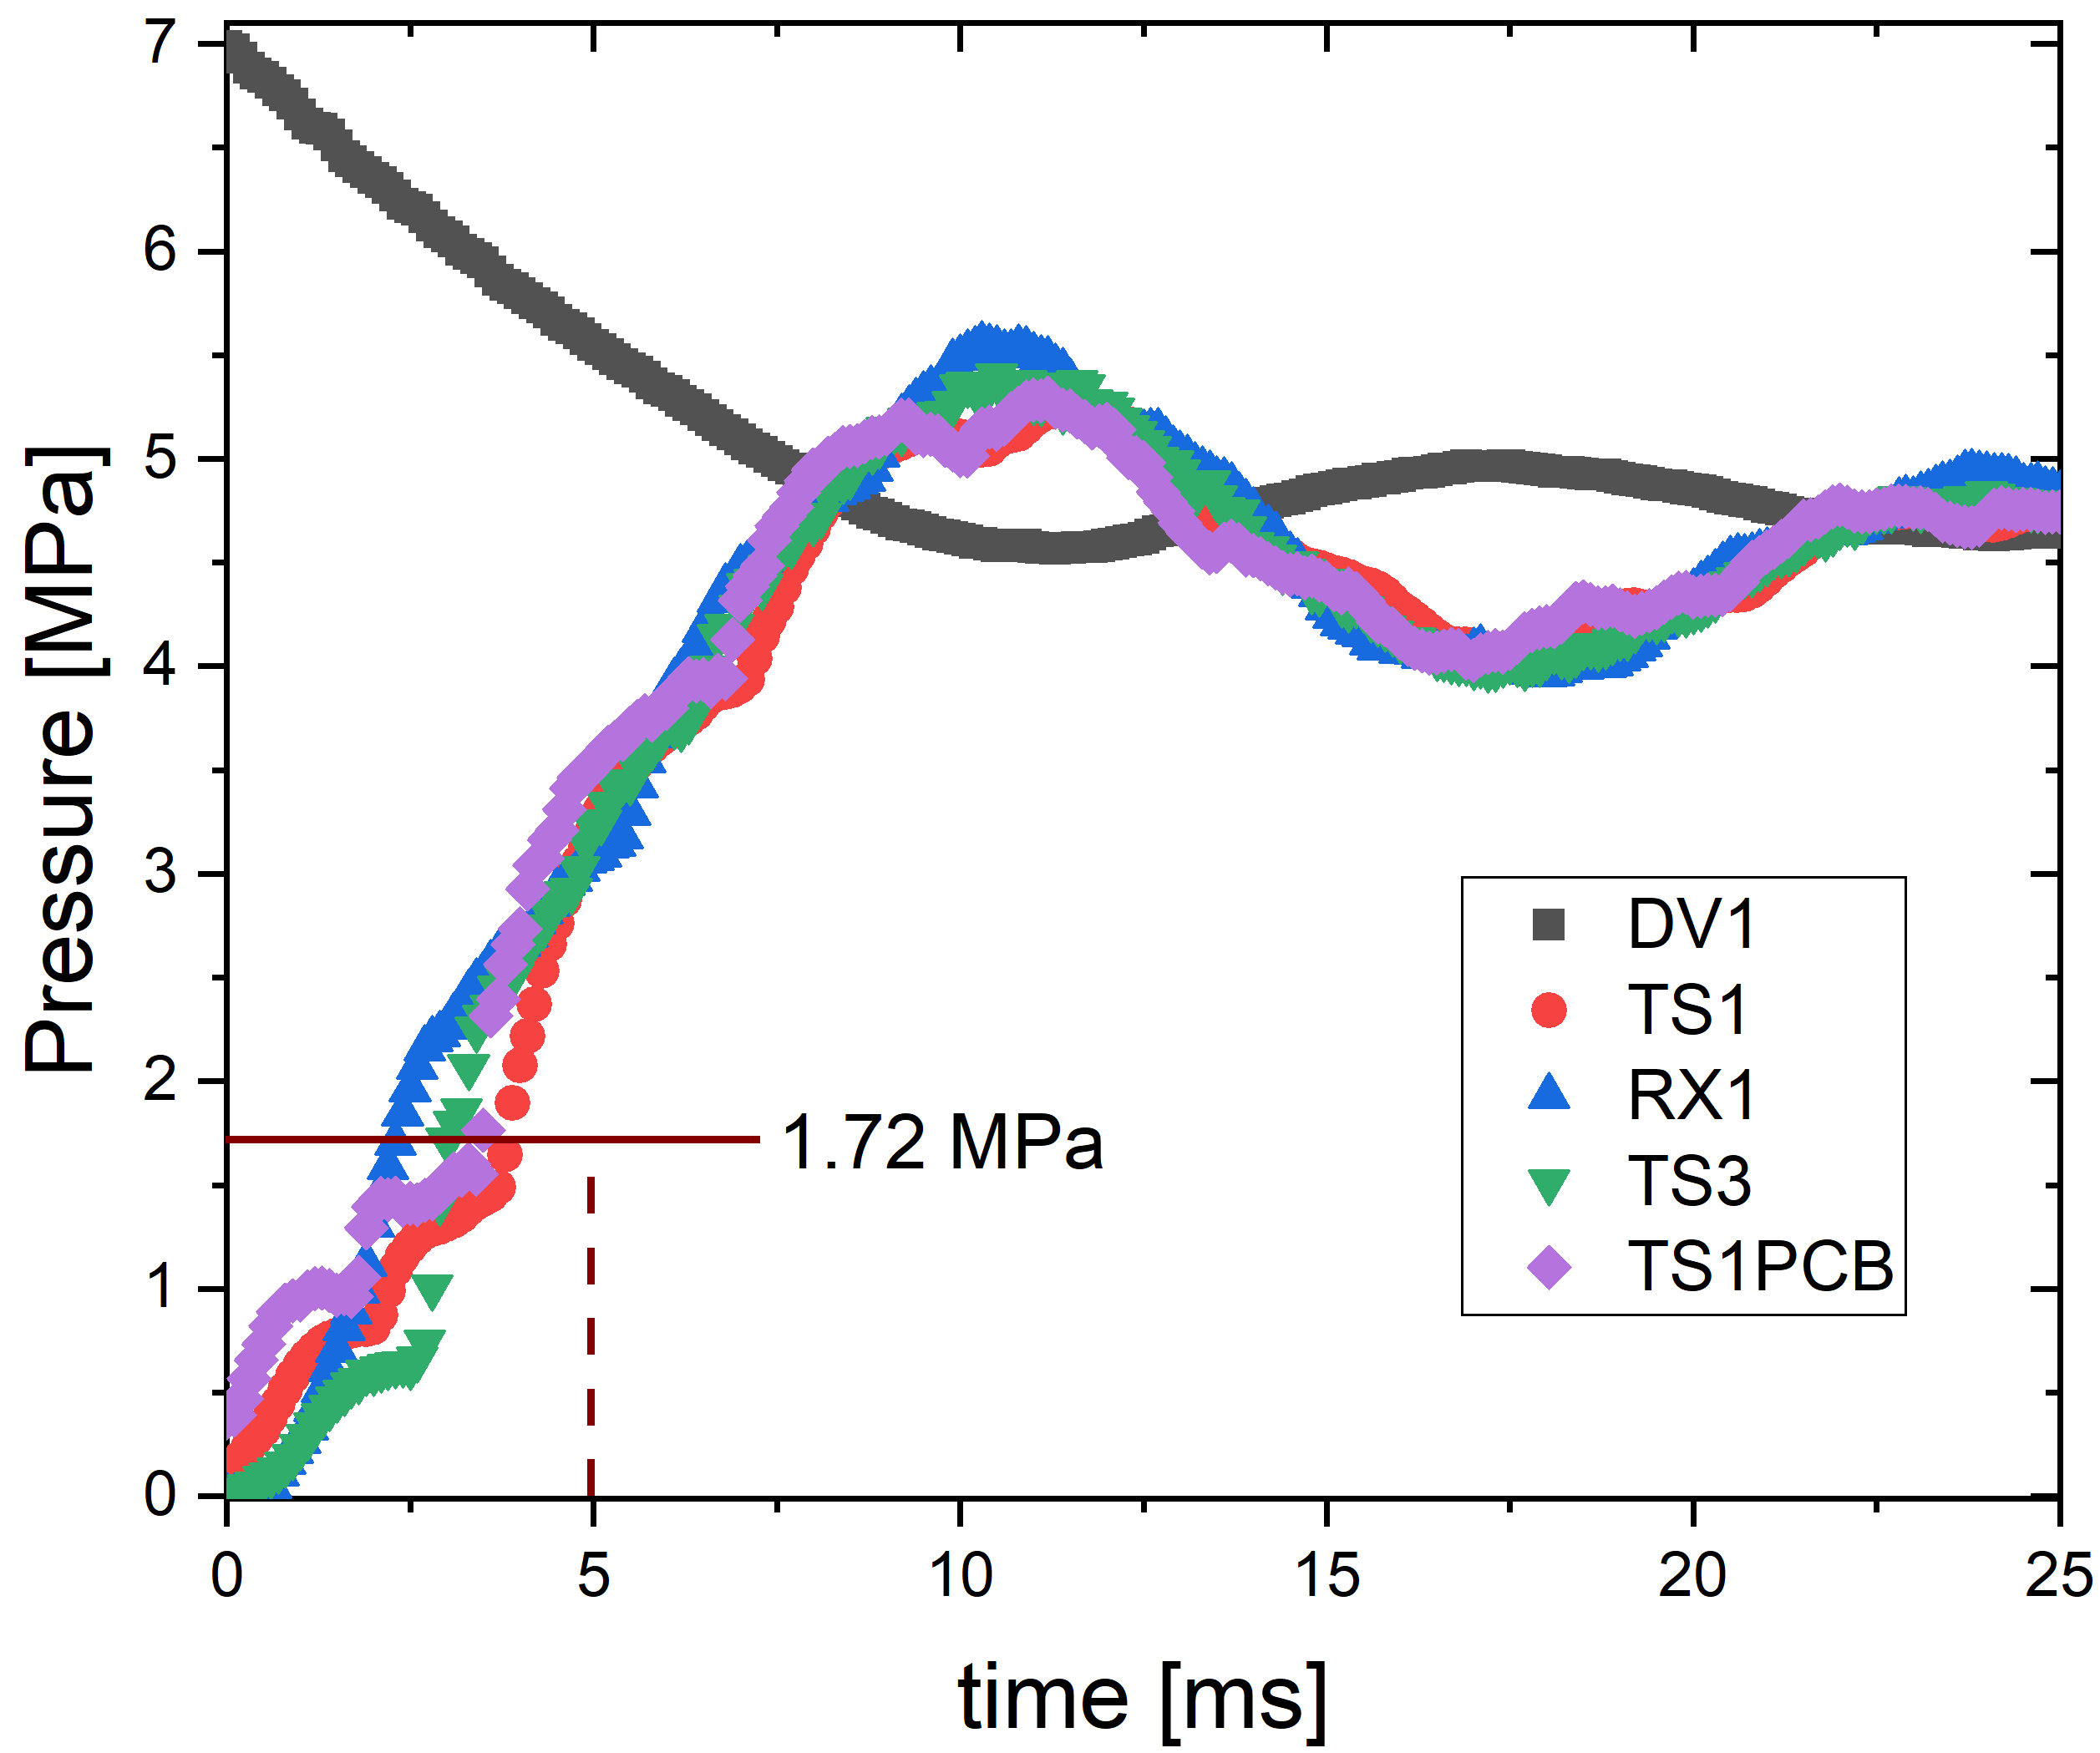
\includegraphics[width=0.9\textwidth]{results/plots/1000psi_annular_BD.png}
        \caption{Pressure over time for a rupture disk HENRI test in an annular test section.}
        \label{fig:ann disk}
    \end{subfigure}
    
    \caption{Results of rupture disk HENRI tests at an initial pressure of \SI{6.9}{\mega\pascal} (\SI{1000}{psia}) and with intermediate tube inner diameter of \SI{2.54}{\centi\meter} (\SI{1}{inch}) for both cylindrical and annular test sections.}
    \label{fig:disk}
    \vspace{16pt}
\end{figure}

The pressure evolution for the HENRI prototype using rupture disks is presented in \Cref{fig:disk}. The cylindrical test section has been selected for the final HENRI design, however, testing was performed with an annular test section to determine if the geometry could meet the pressurization requirements, while reducing the amount of helium-3 that is self-shielded from neutrons by helium-3 closer to the wall. The annular geometry was decided against due to its complexity and reduced pressurization speed. \Cref{fig:ann disk} shows the pressure evolution for the annular geometry using a rupture disk, which is smoother, but slower than the same test performed with the cylindrical geometry, seen in \Cref{fig:cyl disk}.

\subsection{First Piston Valve Design}
% subsection about piston v rupture disk
%\subsection{Piston Valve Compared to Rupture Disk} \label{s:disk v piston}

\begin{figure}[tb]
    \vspace{16pt}
    \centering
    \begin{subfigure}[t]{0.45\textwidth}
        \centering
        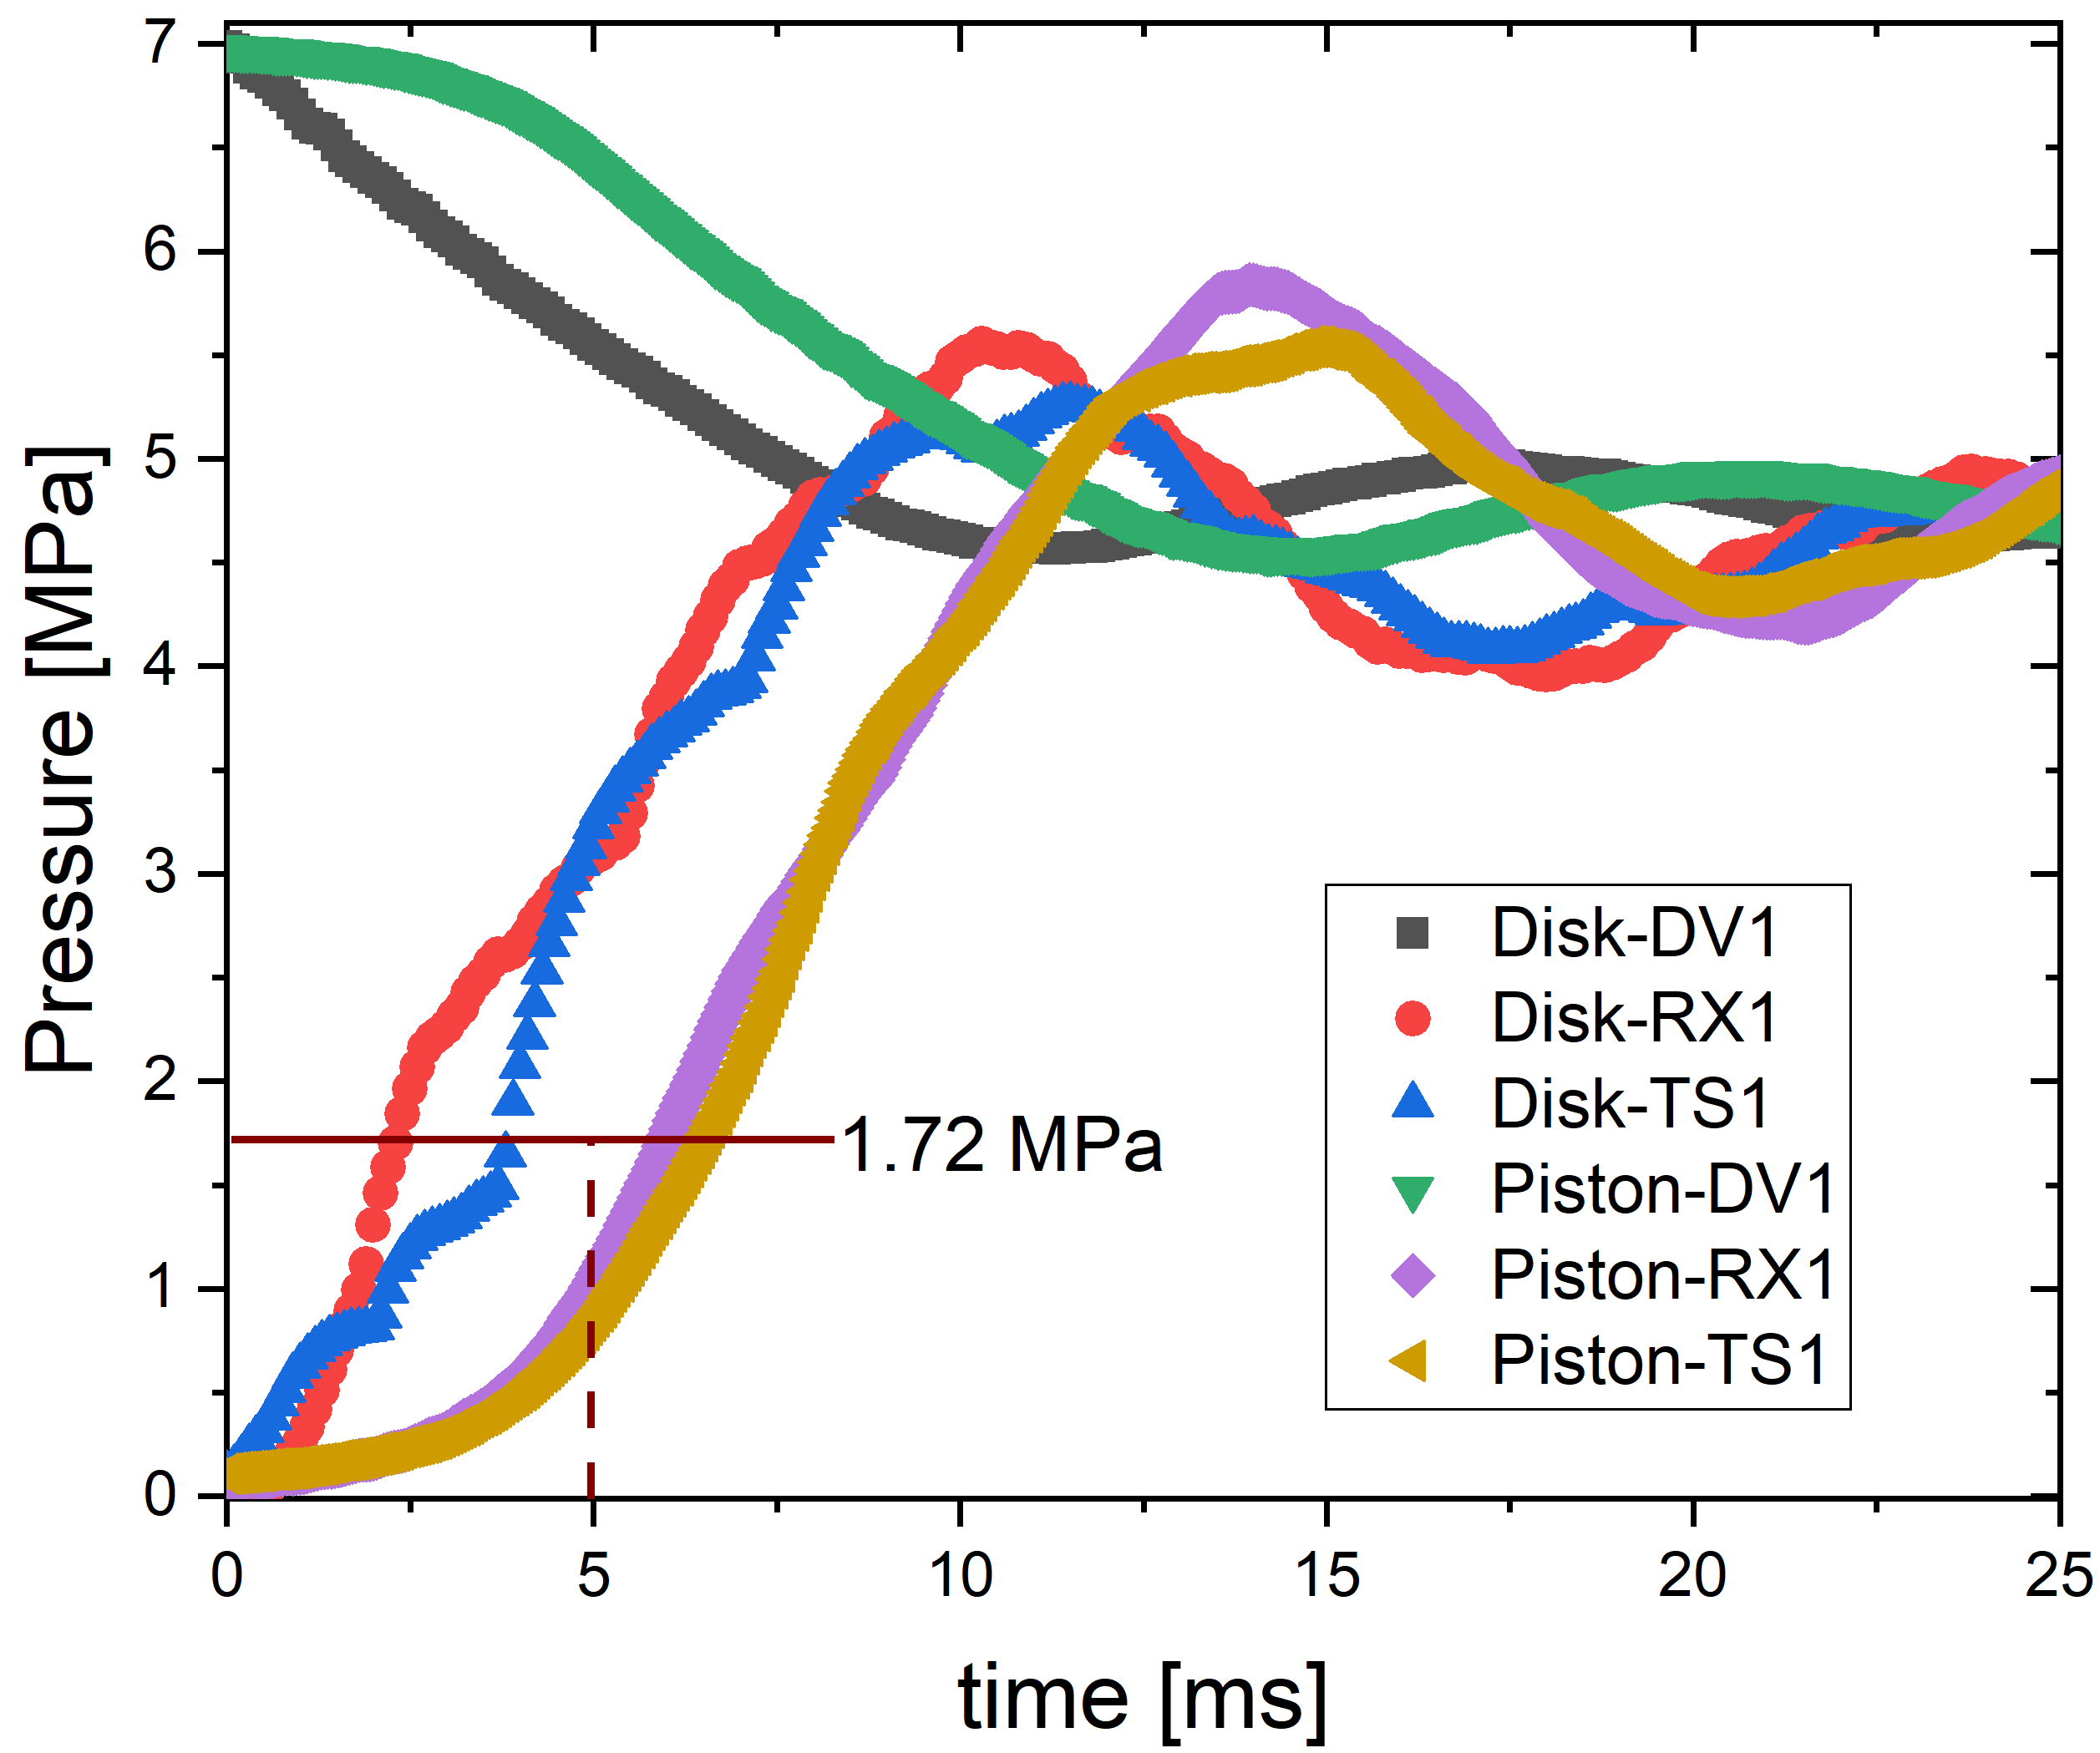
\includegraphics[width=0.9\textwidth]{results/plots/1000psi_annular_BD_Piston.png}
        \caption{Pressure over time for rupture disk HENRI compared to first piston valve design for an annular HENRI test.}
        \label{fig:mtm disk}
    \end{subfigure}
    \hfill
    \begin{subfigure}[t]{0.45\textwidth}
        \centering
        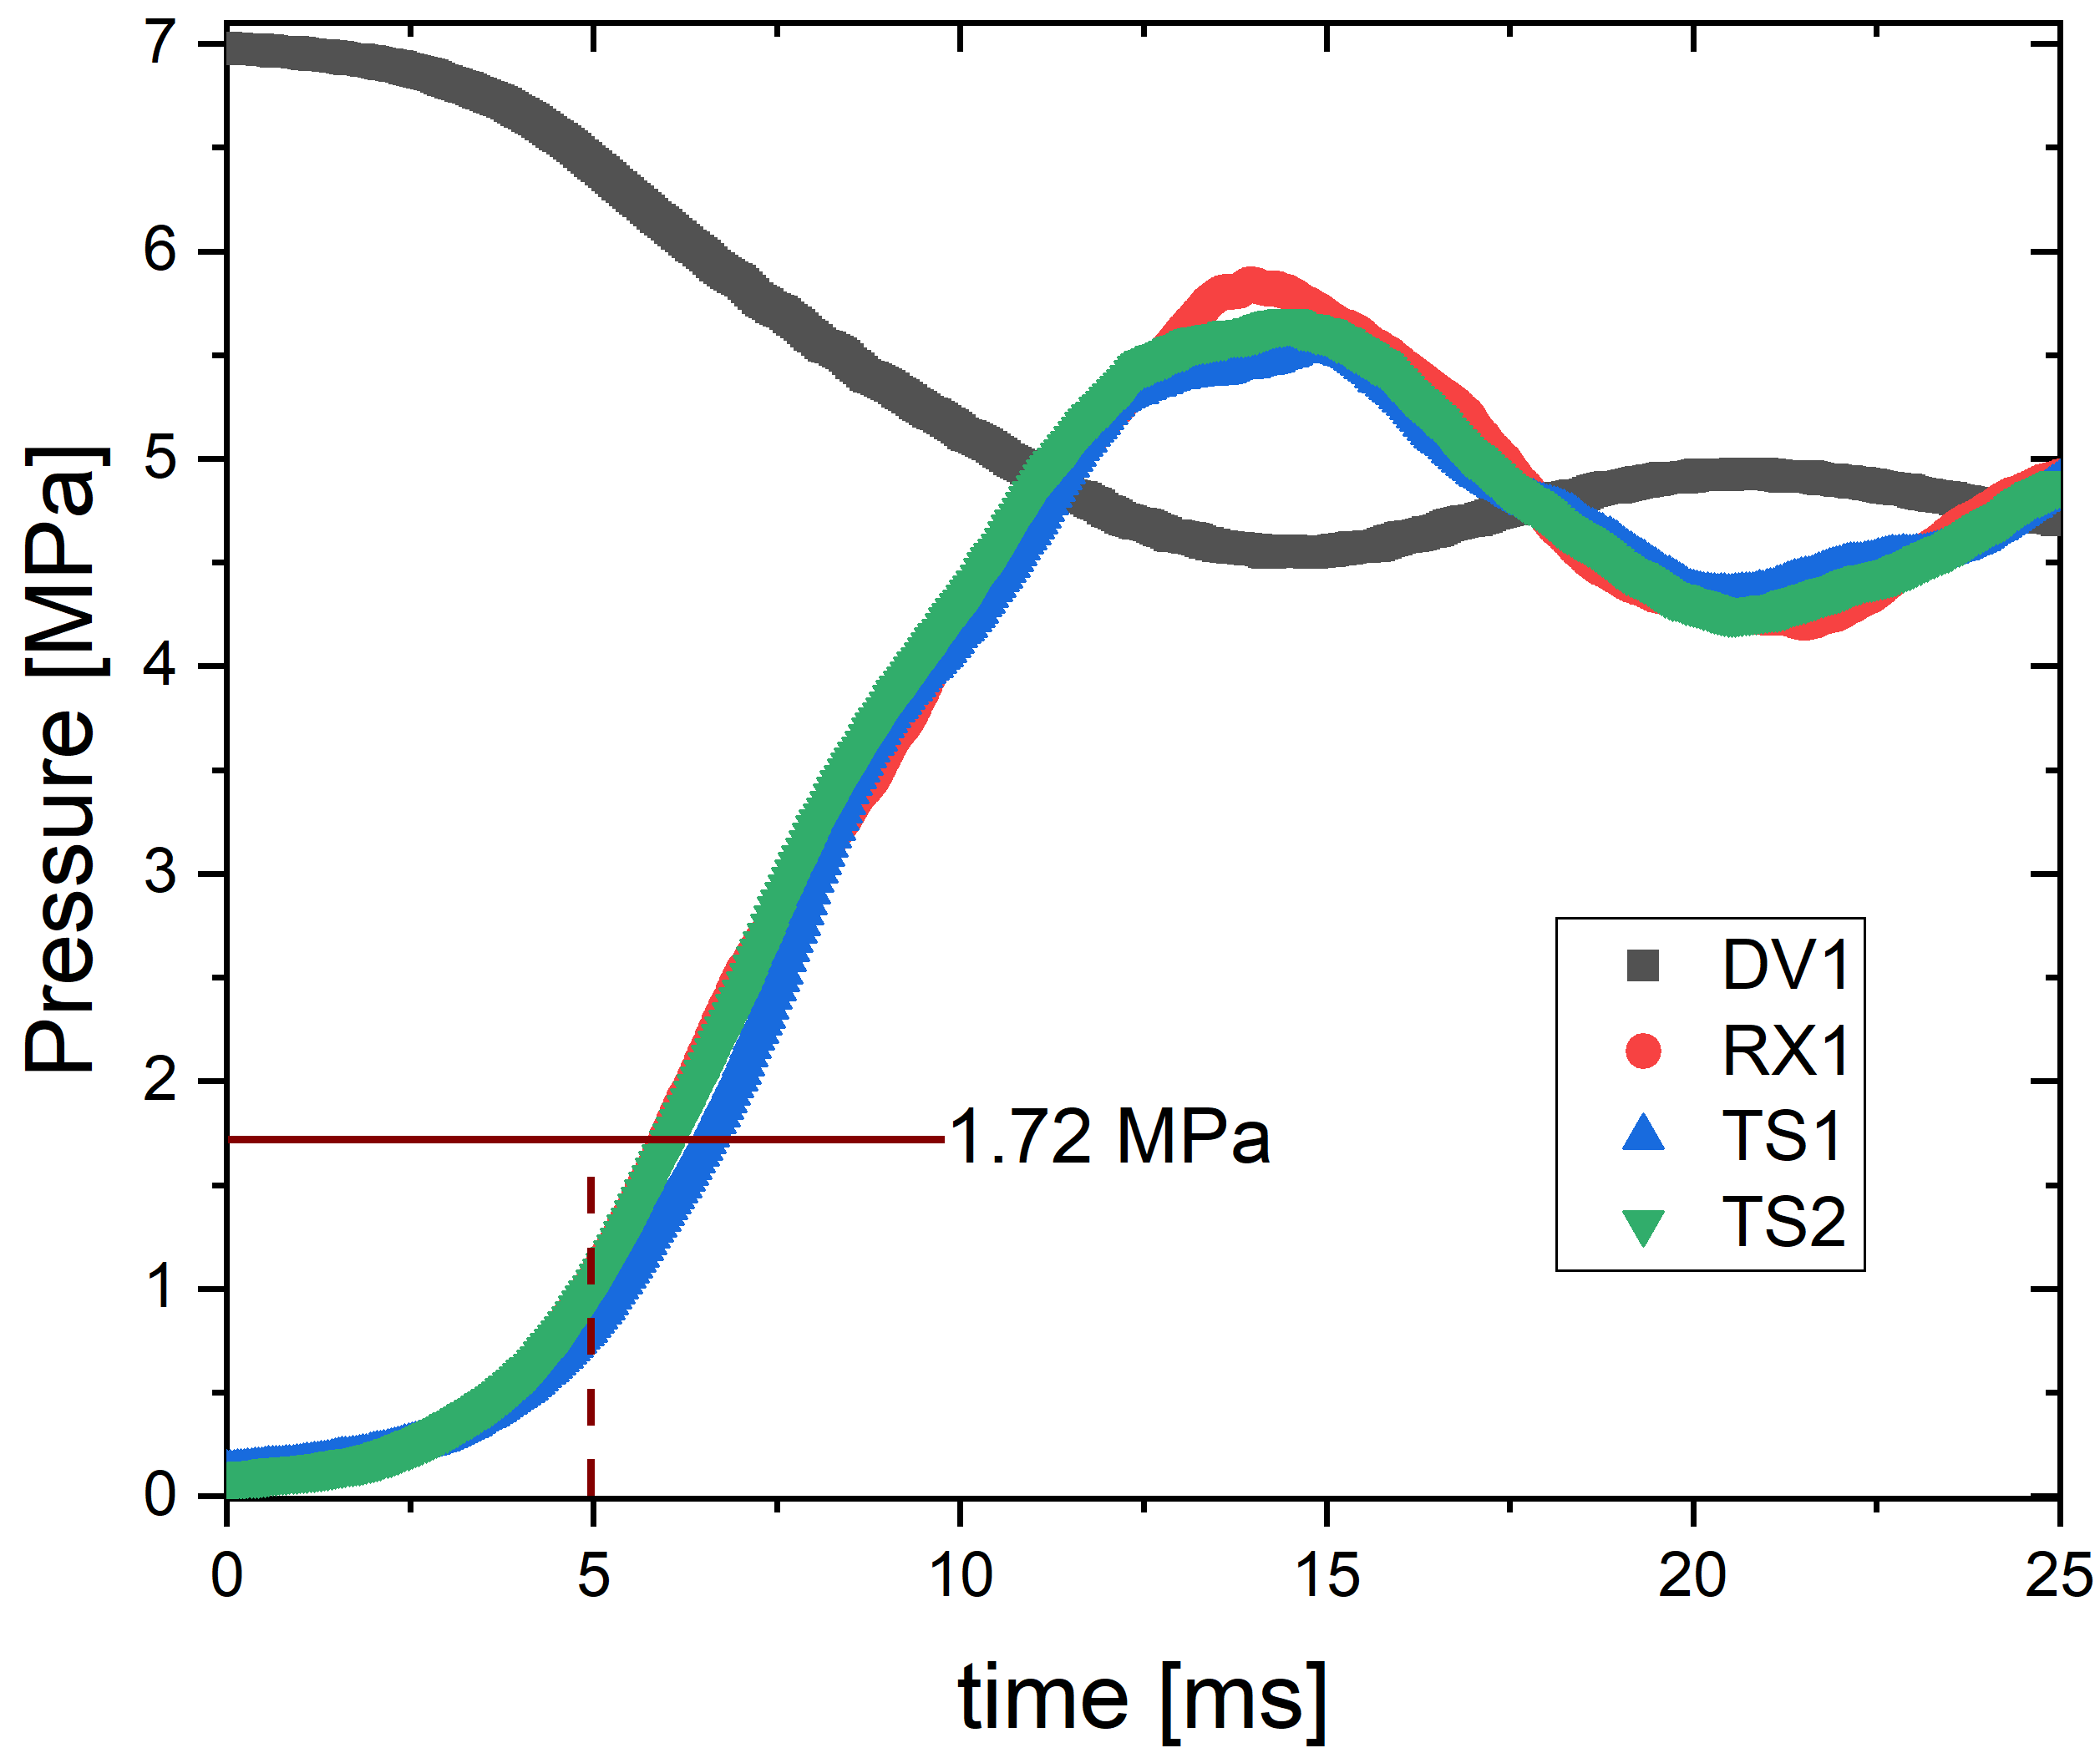
\includegraphics[width=0.9\textwidth]{results/plots/1000psi_MtMseal.png}
        \caption{Pressure over time for the first piston valve design in an annular HENRI test.}
        \label{fig:piston metal 1000psi}
    \end{subfigure}
    
    \caption{Comparison of rupture disk and first piston valve design HENRI tests in an annular test section at an initial pressure of \SI{6.9}{\mega\pascal} (\SI{1000}{psia}) and with intermediate tube inner diameter of \SI{2.54}{\centi\meter} (\SI{1}{inch}).}
    \label{fig:piston v disk}
    \vspace{16pt}
\end{figure}


The rupture disks were used in the HENRI system to determine if the system was capable of pressurizing to \SI{1724}{\kilo\pascal} (\SI{250}{psi}) in the desired time frame of \SI{5}{\milli\second}\cite{HeNURETH}. One of the goals of the piston valve is to open quickly enough to maintain as close to rupture disk physics as possible. 
%Computational fluid dynamics (CFD) simulations were validated using these experiments \cite{CFDNureth,HENRIATH}[MIGHT NEED DIFF REF HERE].
\Cref{fig:piston v disk} compares the results of a rupture disk test and a piston valve test, both with initial driver tank pressure of \SI{6.9}{\mega\pascal} (\SI{1000}{psia}) and intermediate tube inner diameter of \SI{2.54}{\centi\meter} (\SI{1}{inch}). The pressure evolution of the test using the first piston valve design has a slight delay when compared to the results of the rupture disk test. Once the valve is completely open, the evolution matches well, including the shocks travelling back and forth along the test section. However, the valve does not open immediately and there is a small leak from the driver tank to the test section before the top chamber of the piston is fully pressurized and the valve is open. The delay is not ideal, however, with a modification to the design, or adjustment to the timing, it can be mitigated.







% first piston valve design
% the metal to metal seal did not last long -- durability issues, wear on the sealing surface, even with fancy materials; there was a small leak from the driver tank to the test section before the valve was fully open;
%%%%%%%%%%%%%%%%%%%%%%%%%%%%%%%%%%%%%%%%%%%%%%%%%%%%%%%%%%%%%%%%%%%%%%%%%%%%%%%%%%
% subsection about piston valve repeatability
%\subsection{Piston Valve Repeatability} \label{ss:repeatability}


\begin{figure}[b!]
    \vspace{16pt}
    \centering
    \begin{subfigure}[t]{0.45\textwidth}
        \centering
        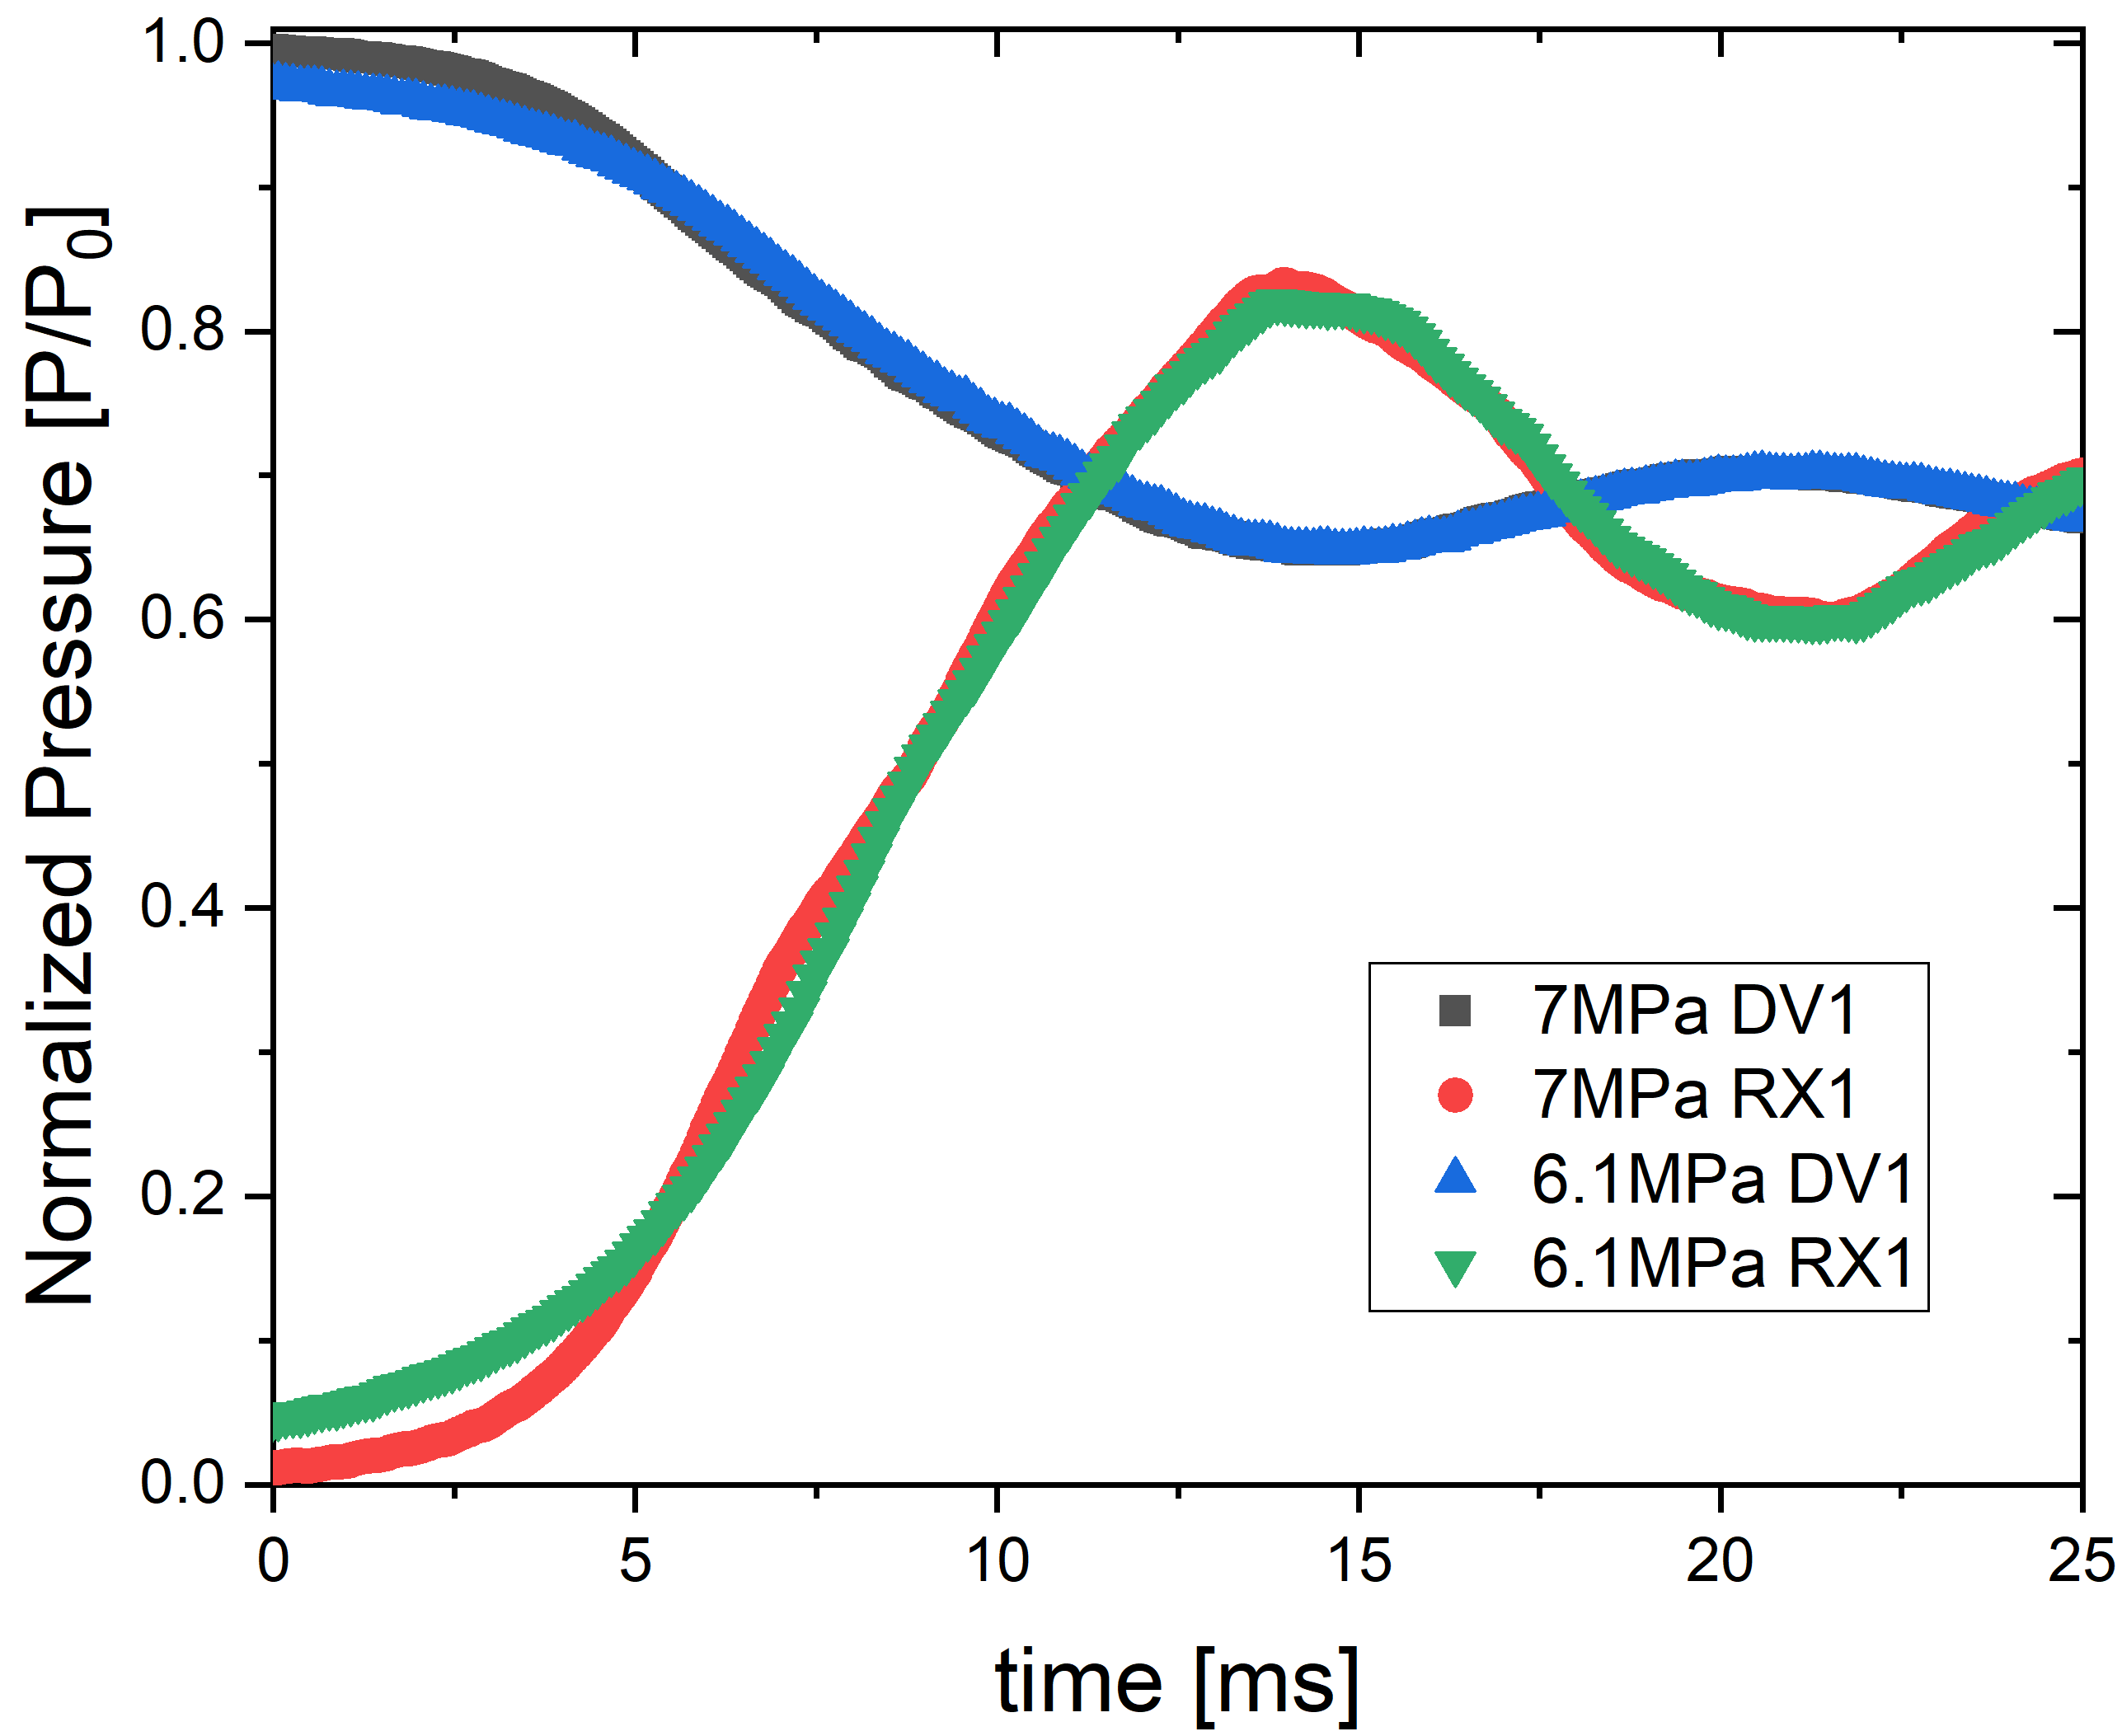
\includegraphics[width=0.9\textwidth]{results/plots/Normalized_RX1_MTM.png}
        \caption{First design piston valve test results normalized by initial driver tank pressure for a range of initial driver tank pressures.}
        \label{fig:norm}
    \end{subfigure}
    \hfill
    \begin{subfigure}[t]{0.45\textwidth}
        \centering
        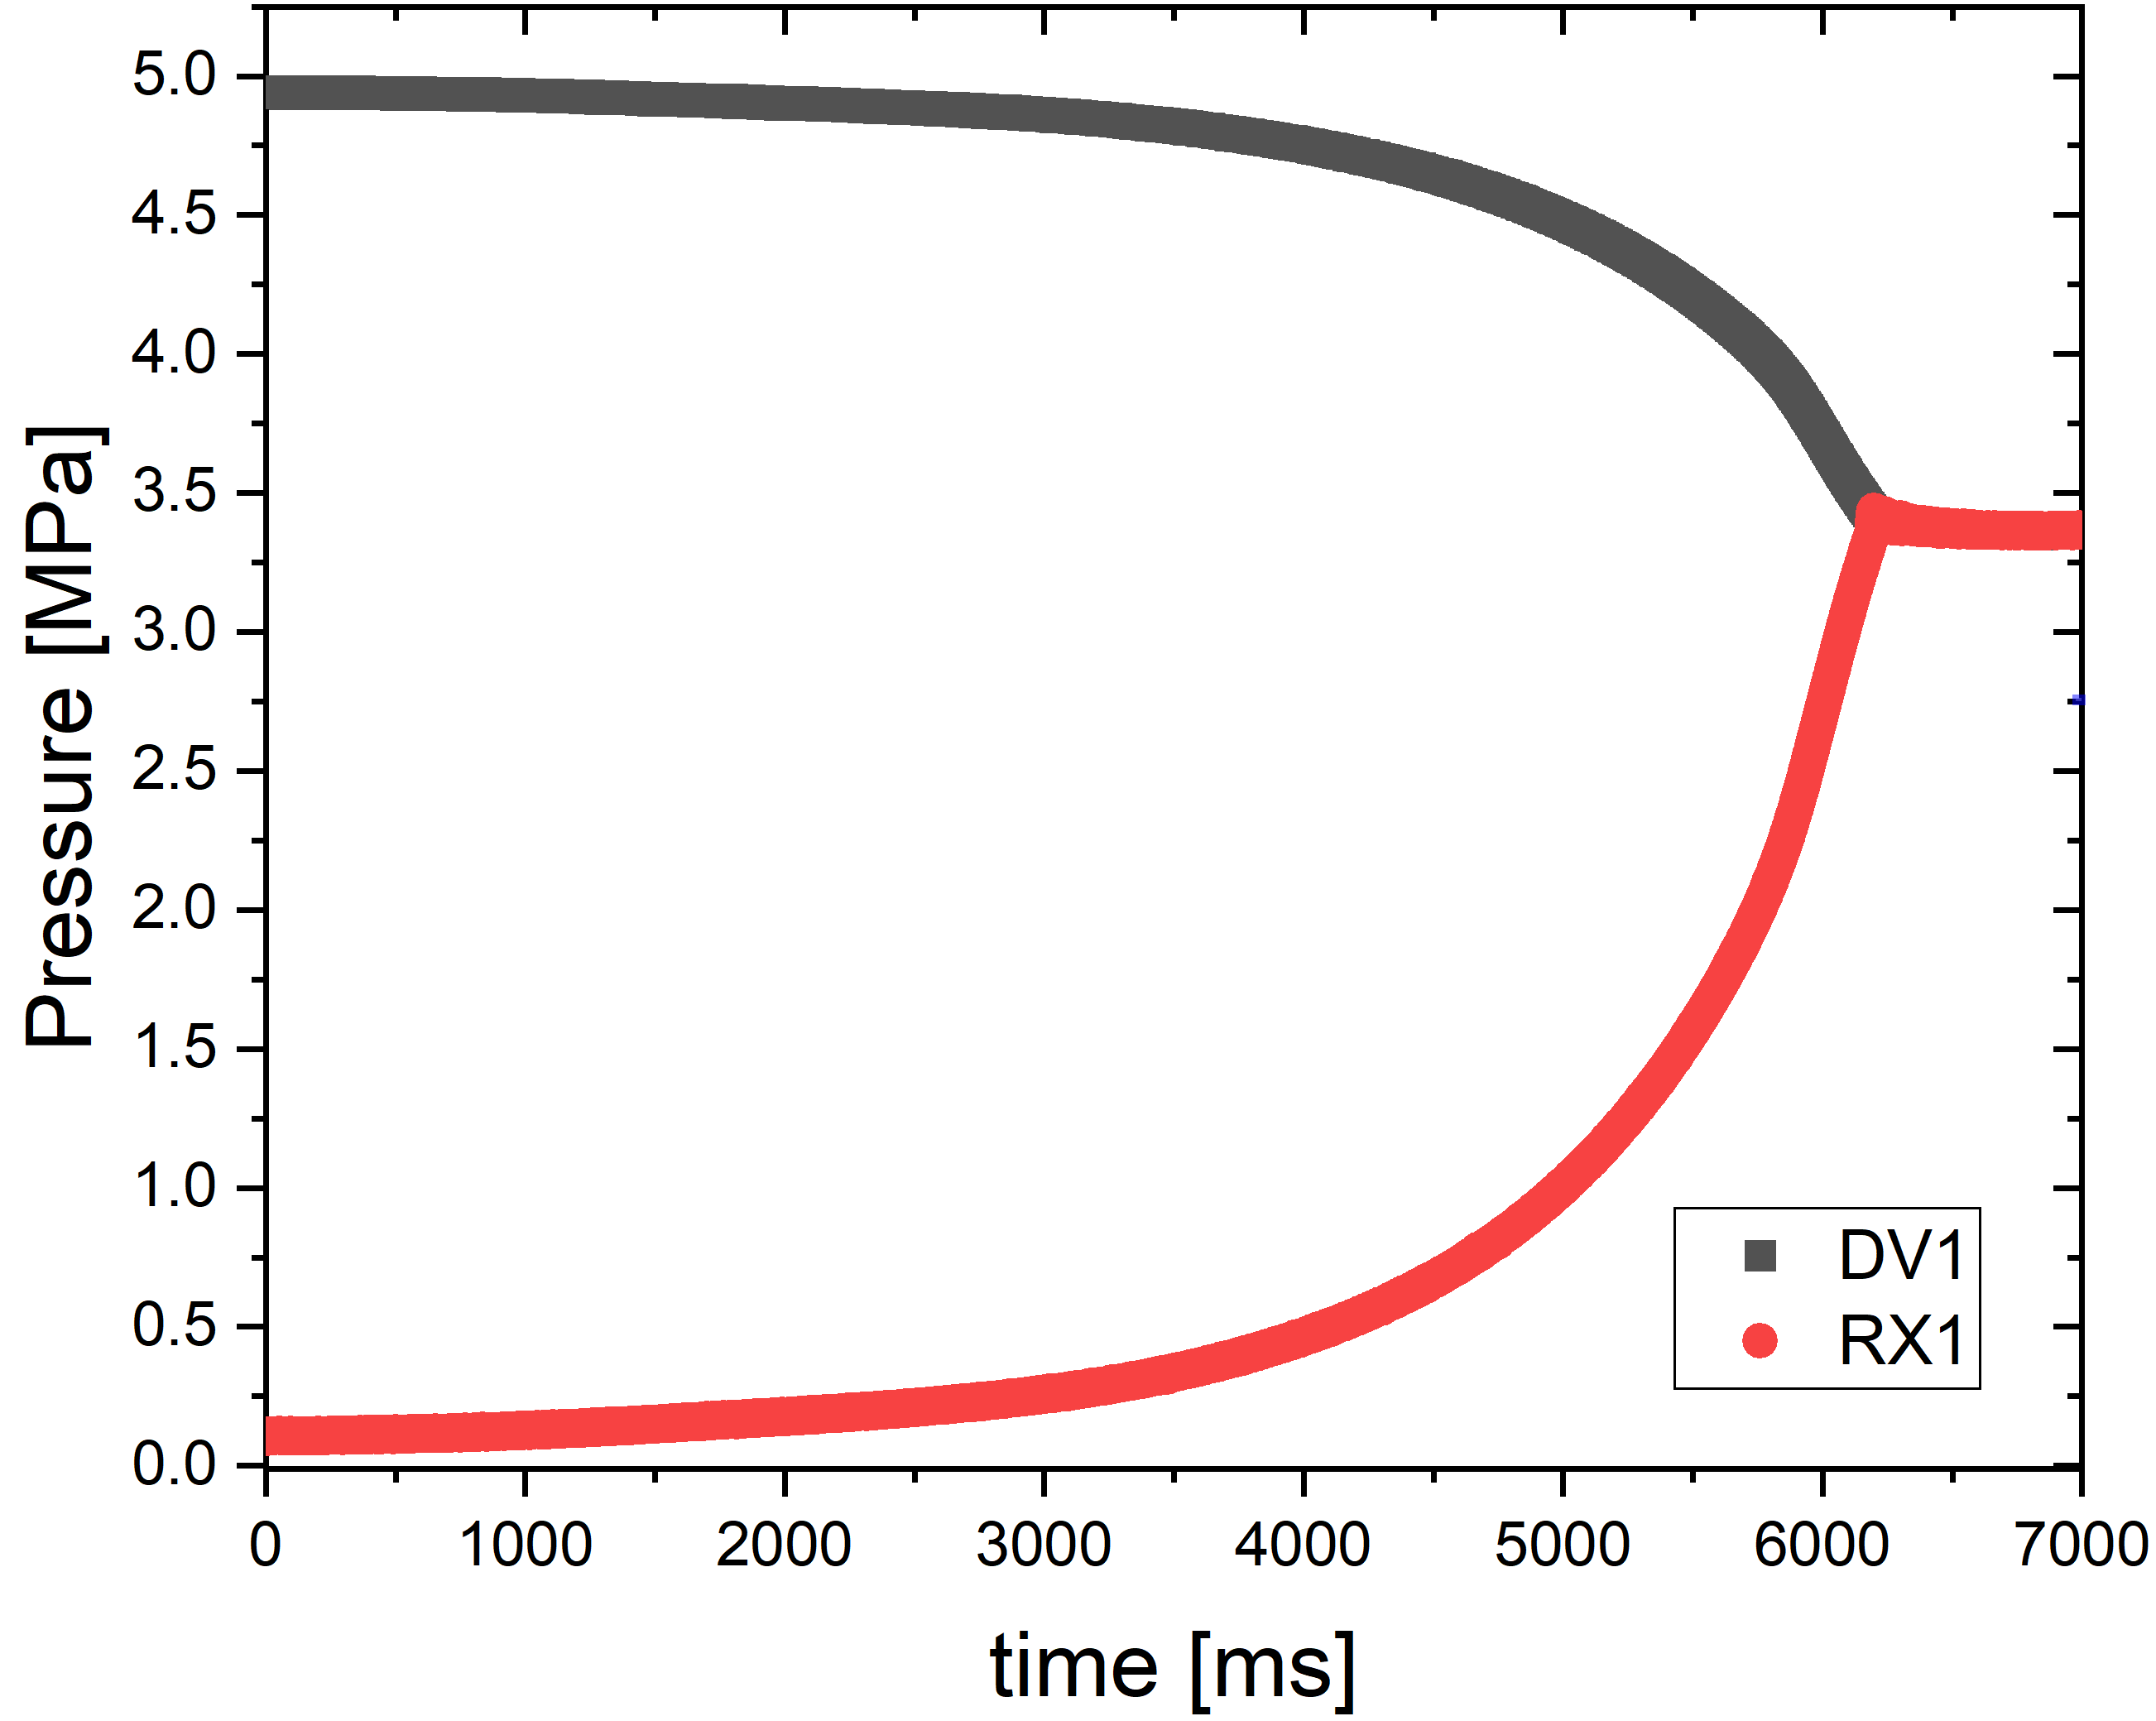
\includegraphics[width=0.9\textwidth]{results/plots/718psi_MtM_annular.png}
        \caption{First design piston valve test with a seal failure at an initial pressure of \SI{4.96}{\mega\pascal} (720 psi).}
        \label{fig:piston 2 test}
    \end{subfigure}
    \caption{Comparison of results for first piston valve that demonstrate poor repeatability and low pressure sealing ability.}
    \label{fig:piston repeatability}
    \vspace{16pt}
\end{figure}


The valve selected for the HENRI system must provide a repeatable and predictable pressurization of the cartridge during a TREAT transient. \Cref{fig:norm}, shows two tests with the first piston valve design at two pressures: \SI{7}{\mega\pascal} (1000psi) and \SI{6.1}{\mega\pascal} (890psi), normalized by initial driver tank pressure. There is a slight delay in the second test compared to the first test, but after the delay, the results match closely. This comparison demonstrates the first piston valve's need for high pressure to maintain a seal. With less pressure in the driver tank, the plug is not held against the flange as tightly and some helium is able to leak through before the piston has moved the plug fully away from the flange. The second plot, \Cref{fig:piston 2 test}, shows a test using the first piston valve design in which the seal failed before the valve was opened. In preparation for a test at \SI{4.96}{\mega\pascal} (720 psi), the piston valve is closed, but does not hold the seal and a leak develops between the driver tank and the test section. The seal plug used in this test is too worn and cannot hold a seal. The durability of the piston valve must be tested to find the operation limit.


%%%%%%%%%%%%%%%%%%%%%%%%%%%%%%%%%%%%%%%%%%%%%%%%%%%%%%%%%%%%%%%%%%%%%%%%%%%%%%%%%%
% subsection about seal durability testing on the piston valve
%\subsection{Piston Valve Re-usability} \label{ss:reusability}

\begin{figure}[tb]
    \vspace{16pt}
    \centering
    \includegraphics[width=0.9\textwidth]{design/photos/plug_gen1_wear_crop_labels.png}
    \caption{Plugs for piston valve. Left to right: stainless steel, stainless steel, and aluminum.}
    \label{fig:plug wear}
    \vspace{16pt}
\end{figure}

The re-usability of the piston valve was tested by cycling the piston 500 times, then comparing the sealing capability to before the cycles. After 500 cycles, the piston valve would not hold a seal, even with over \SI{6.9}{\mega\pascal} (1000 psi) in the bottom chamber of the piston and in the driver tank. The valve needs to be used without being replaced or maintained often, which is one of the reasons the rupture disks do not work. The metal plug was observed to have significant wear after the cycling tests, seen in \Cref{fig:plug wear}, which was asymmetrical. The used stainless steel plug, left, has extreme asymmetrical wear, which meant that the plug could not be used to seal at any pressure. The wear on the aluminum plug was also asymmetrical, however the softer metal was worn more easily and the plug has a more defined ring around its circumference. Not shown is a cobalt alloy plug that was tested to see if a harder metal would better resist wear and maintain a seal for longer. However, the asymmetrical wear degrades the seal, even with little wear visible on the plug. The asymmetrical wear was attributed to the three legged piston mount that allowed the piston to move slightly in one direction when the valve closed with the piston in extension. A new mount and a new plug design that does not wear as much, and can seal at lower pressures would improve the piston valve design.



%%%%%%%%%%%%%%%%%%%%%%%%%%%%%%%%%%%%%%%%%%%%%%%%%%%%%%%%%%%%%%%%%%%%%%%%%%%%%%%%%%
% subsection about new piston valve design
\subsection{Piston Valve Design Improvements} \label{ss:new valve}



An improved design must have a more robust seal and sealing surface that can seal under a wider range of conditions, and does not degrade as quickly. The piston mount was redesigned to be as symmetrical as possible. The three legs were replaced by a single piece cylinder sandwiched by two plates. One plate attaches the cylinder to the piston and the other plate attaches the cylinder to the flange. The new mount can be seen in \Cref{fig:cad mount 2}. The new plug design has a dovetail groove to hold an o-ring, which is expected to seal at much lower pressures and maintain better sealing capability after many cycles than when compared to the metal-to-metal seal of the first piston valve design. \Cref{fig:plug v2 draw} shows a drawing of the new plug design with the dovetail groove and the relative position of the flange sealing surface. Two different o-rings were selected based on their helium leak rates, high temperature rating, and radiation damage resistance: a FFKM o-ring manufactured by Marko Rubber and a Nitrile o-ring manufactured by Parker. Both o-rings are Shore A 80 hardness, with \SI{0.3531}{\centi\meter} (0.139 inch) cross section, \SI{3.134}{\centi\meter} (1.234 inch) inner diameter, and \SI{3.840}{\centi\meter} (1.512 inch) outer diameter.

\begin{figure}[t!]
    \vspace{16pt}
    \centering
    \begin{subfigure}[t]{0.45\textwidth}
        \centering
        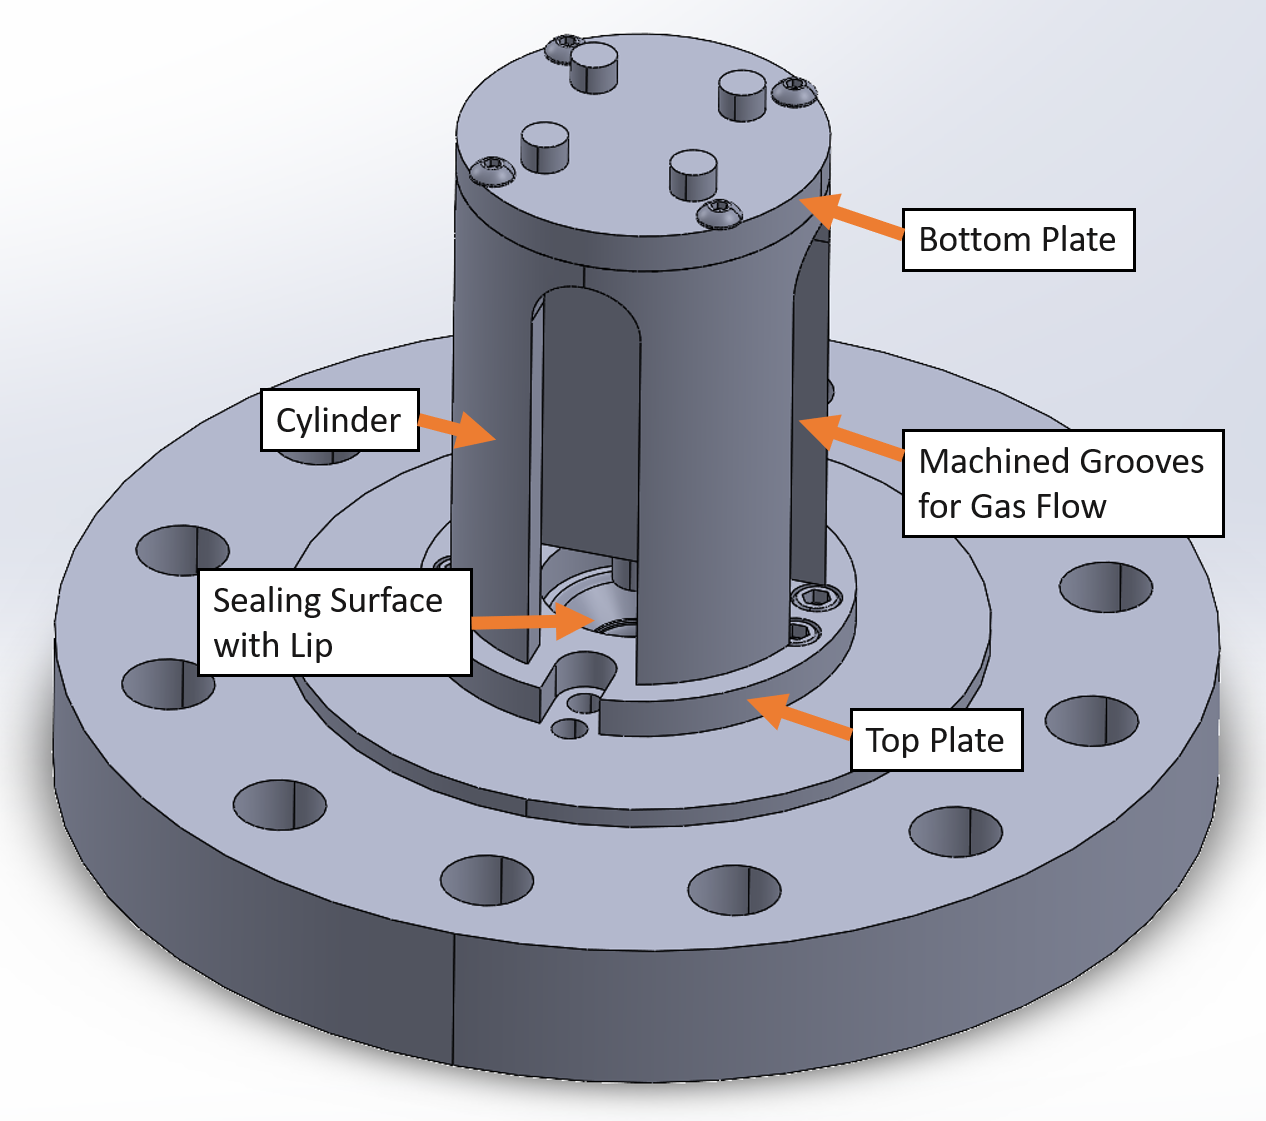
\includegraphics[width=0.88\textwidth]{design/photos/piston_mount_gen2_cad_labels.png}
        \caption{CAD model of cylindrical piston mount on flange.}
        \label{fig:cad mount 2}
    \end{subfigure}
    \hfill
    \begin{subfigure}[t]{0.49\textwidth}
        \centering
        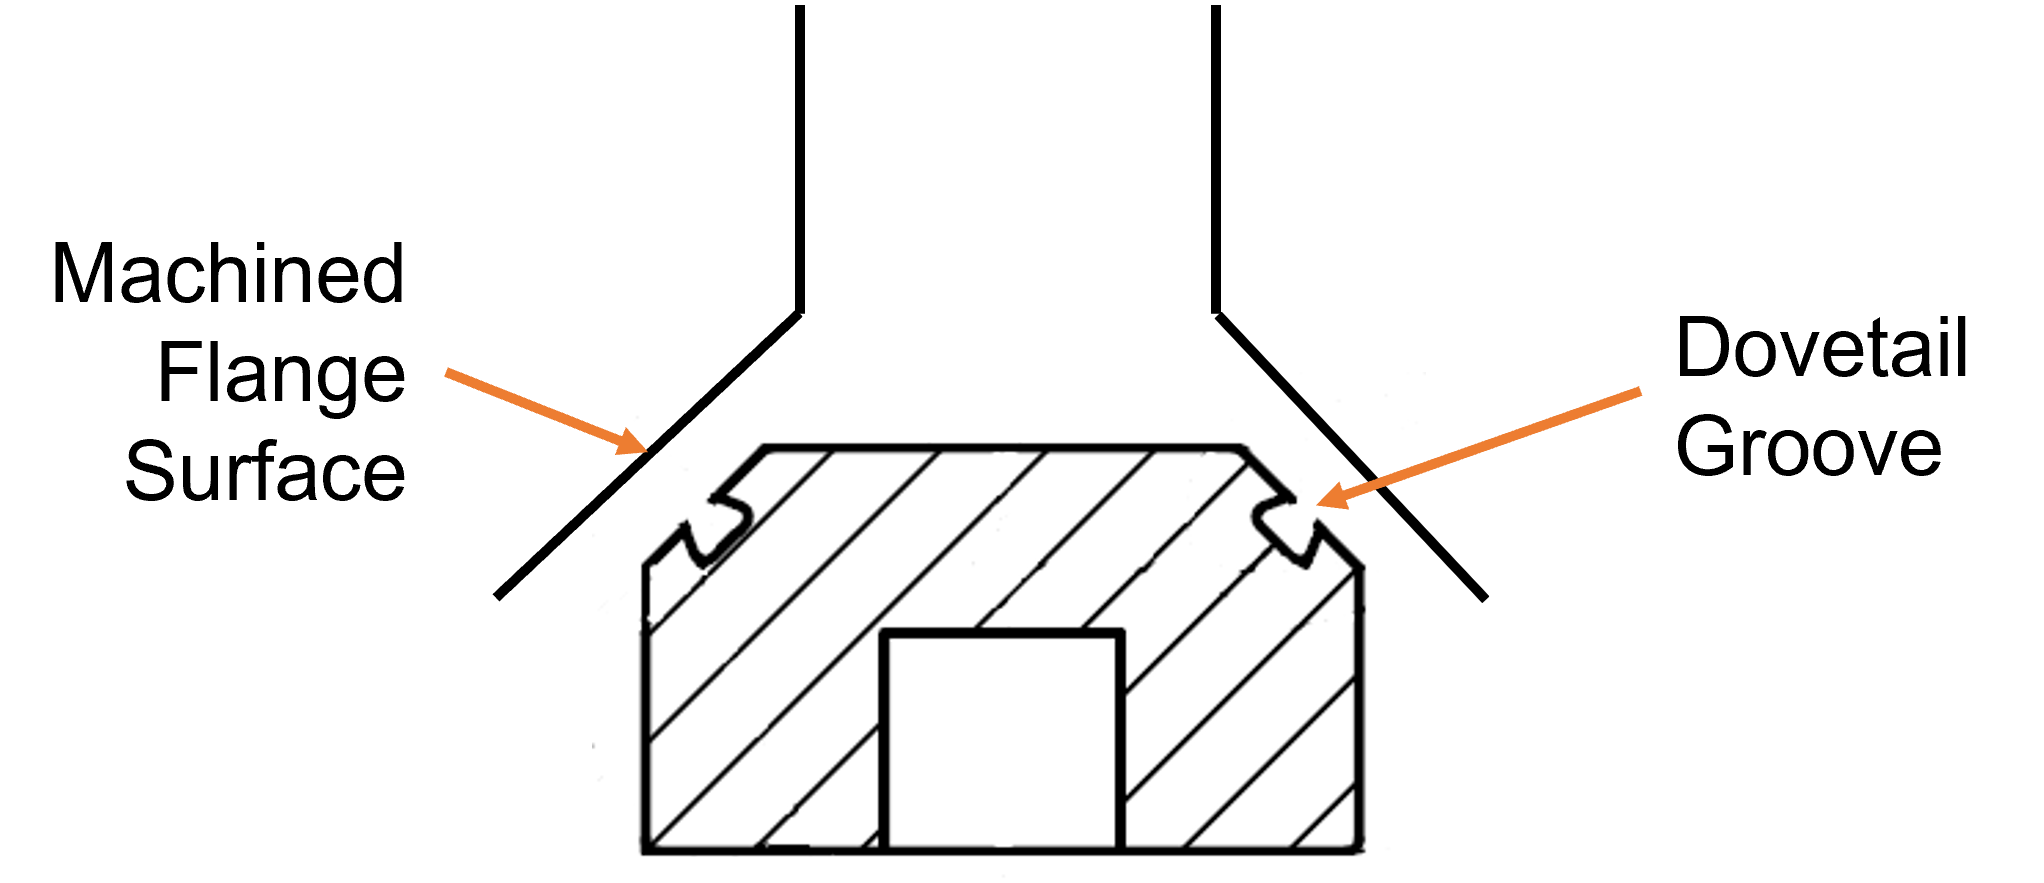
\includegraphics[width=\textwidth]{design/photos/new_plug_draw_crop_paint_labels.png}
        \caption{Drawing of new plug design for piston valve with dovetail groove for an o-ring.}
        \label{fig:plug v2 draw}
    \end{subfigure}
    
    \caption{Redesigned piston valve mount and plug.}
    \label{fig:redesign}
    \vspace{16pt}
\end{figure}

%%%%%%%%%%%%%%%%%%%%%%%%%%%%%%%%%%%%%%%%%%%%%%%%%%%%%%%%%%%%%%%%%%%%%%%%%%%%%%%%%%

\subsection{Improved Piston Valve Design}
% subsection about new piston compared to rupture disk
%\subsection{Improved Piston Valve Compared to Rupture Disk} \label{ss:new piston v disk}



Since a new piston mount and plug have been designed, the new setup needs to be tested and compared to the rupture disk results to ensure the valve is performing adequately and the desired pressure of \SI{1.72}{\mega\pascal} (250 psi) in less than \SI{5}{\milli\second} is still reached. \Cref{fig:disk new} shows a rupture disk and a piston valve test both starting at \SI{6.9}{\mega\pascal} (1000 psi), with a \SI{2.54}{\centi\meter} (1 inch) inner diameter intermediate section. The pressure evolution of the piston valve follows very closely to the rupture disk and the desired pressurization is reached. Also, the same shock structure is observed in the piston valve results, which proves the piston valve is able to open as rapidly as is required. \Cref{fig:piston 1000psi 25ms} shows a piston valve test under the same conditions, but has more instrumentation included. Comparing this plot to \Cref{fig:disk} shows that the piston valve produces pressure and density waves very similar to those of the rupture disk. The new piston valve design improves on the previous design by strongly reducing the observed delay at the beginning of the injection. The first piston valve design produced results, \Cref{fig:piston v disk}, that have a slow leak of pressure before the valve is fully open. The improved piston valve design does not exhibit this behavior. In \Cref{fig:disk new}, there is a small difference in slope at the beginning of the pressurization in the TS3 data between the rupture disk and the improved piston valve. 


\begin{figure}[bt]
    \vspace{16pt}
    \centering
    \begin{subfigure}[t]{0.45\textwidth}
        \centering
        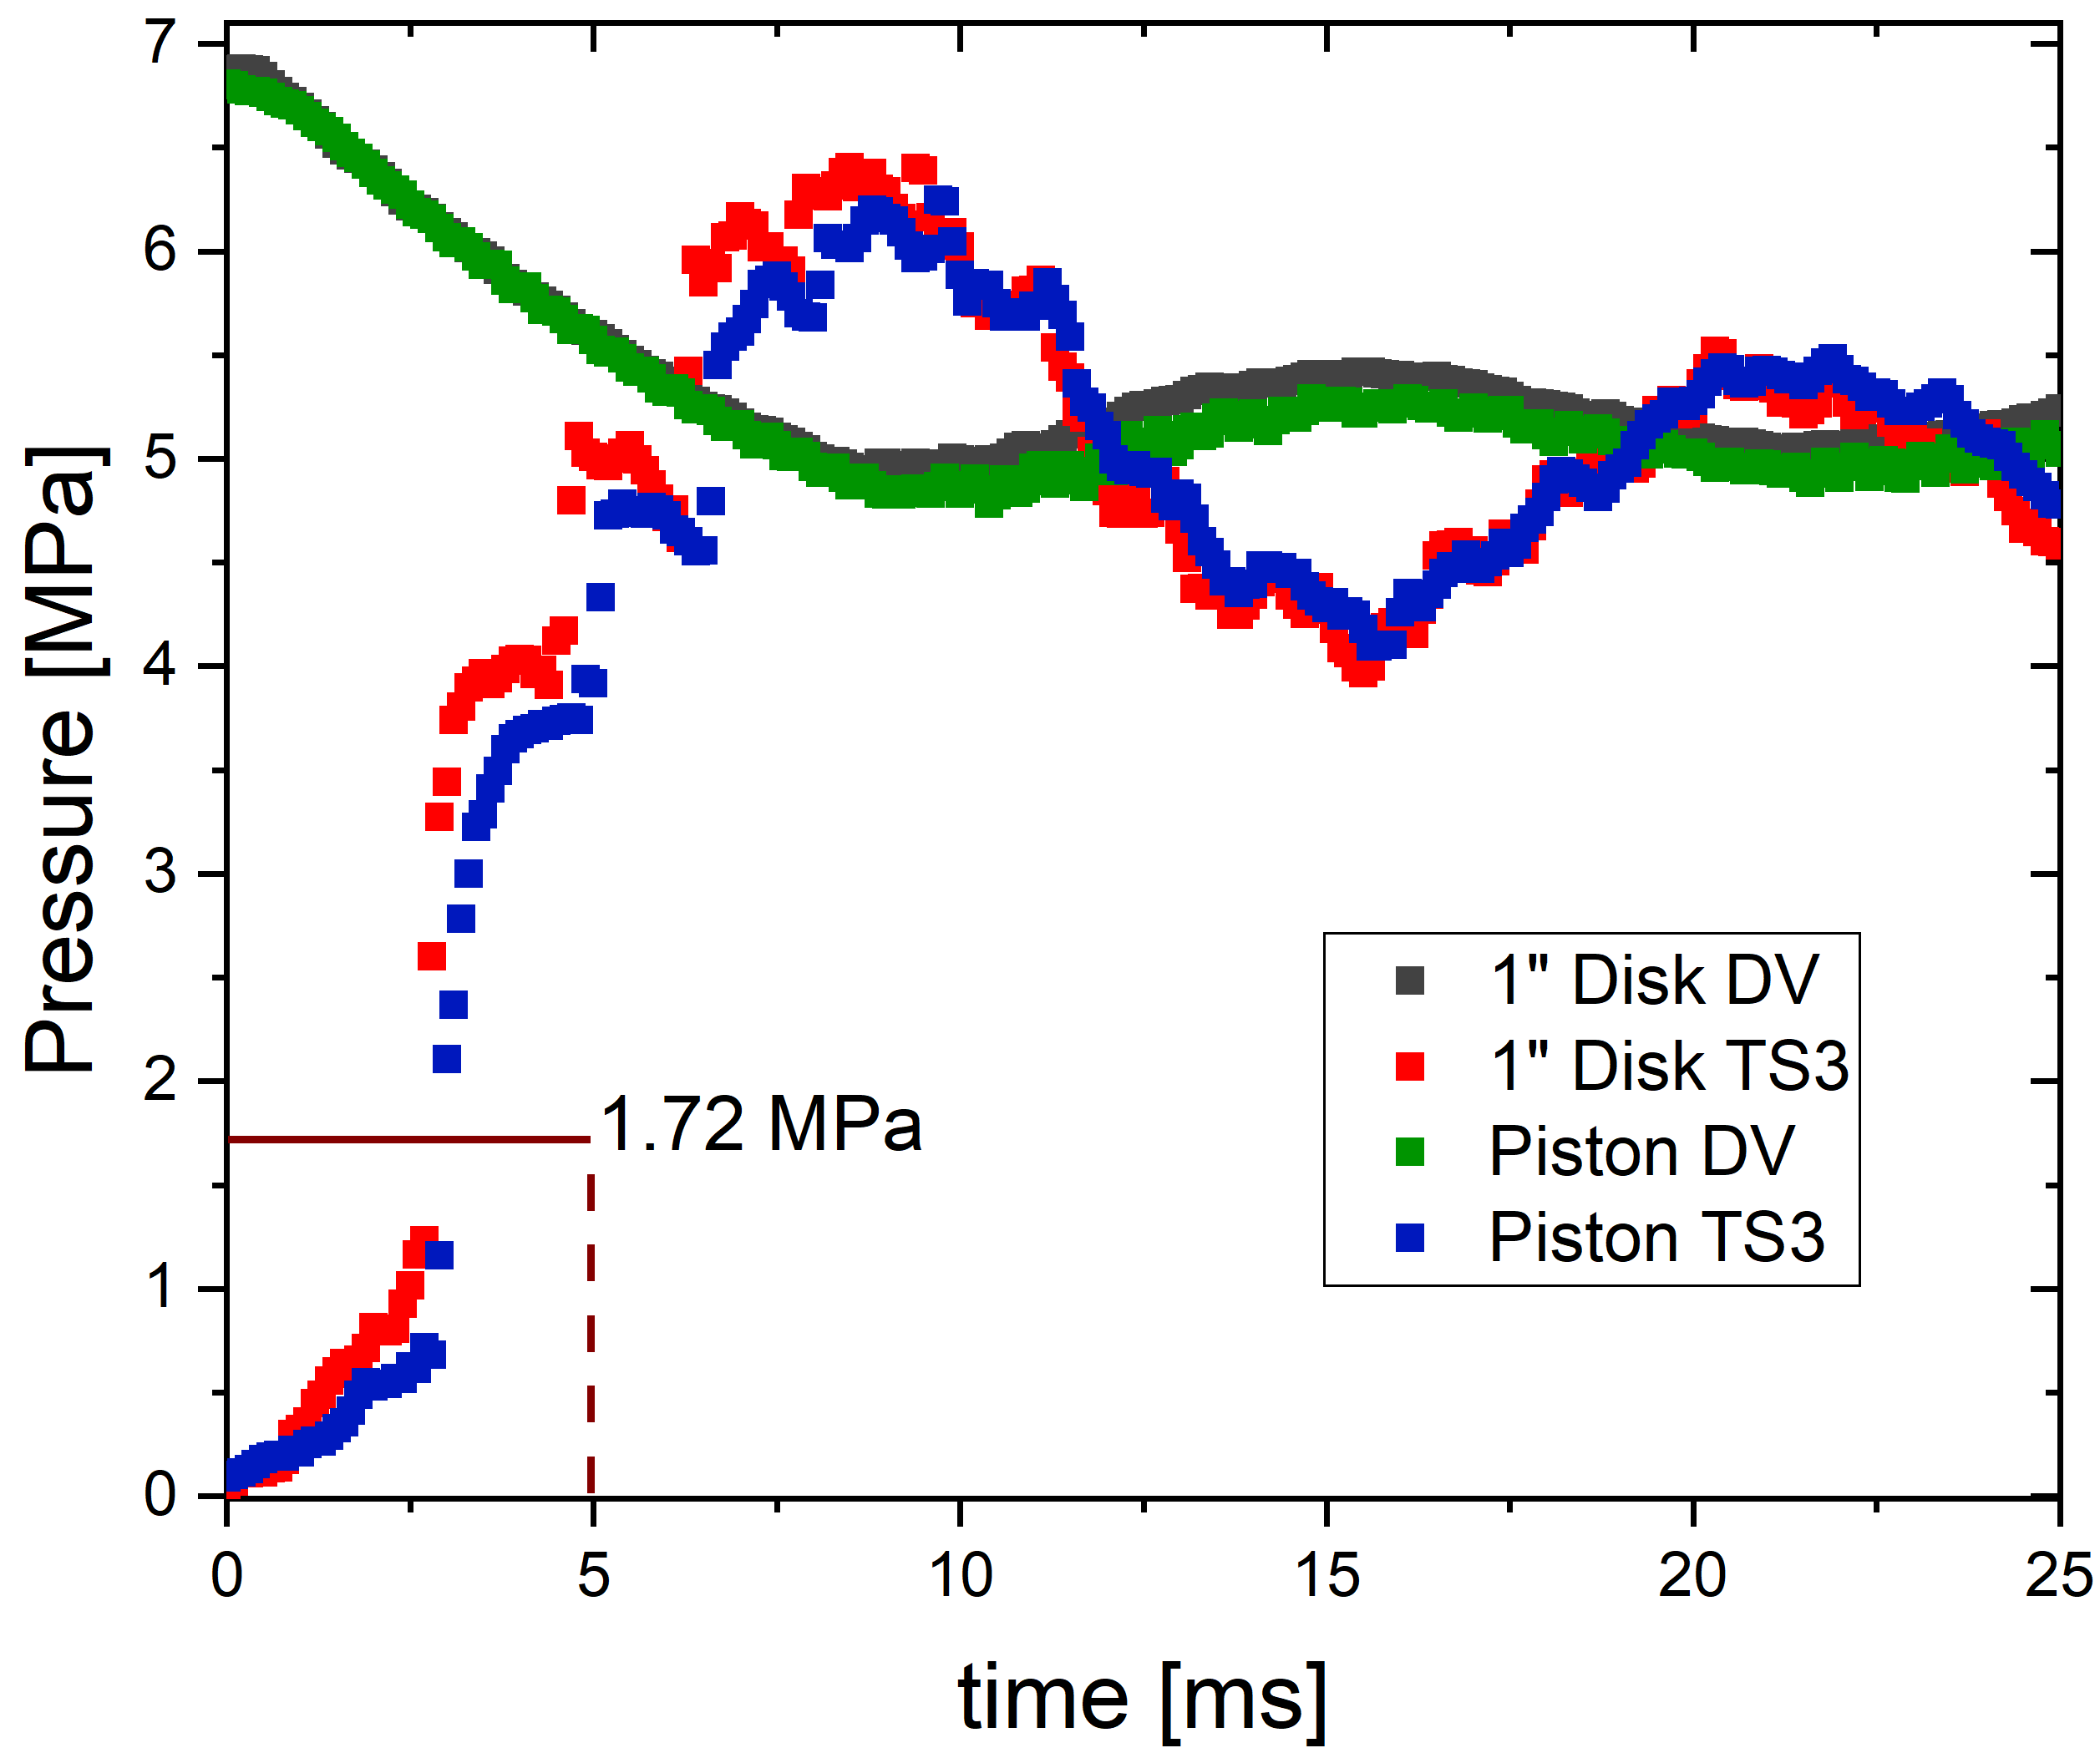
\includegraphics[width=0.9\textwidth]{results/plots/BD_Piston_overlay_1000.png}
        \caption{Pressure over time for rupture disk compared to the second generation plug design HENRI test.}
        \label{fig:disk new}
    \end{subfigure}
    \hfill
    \begin{subfigure}[t]{0.45\textwidth}
        \centering
        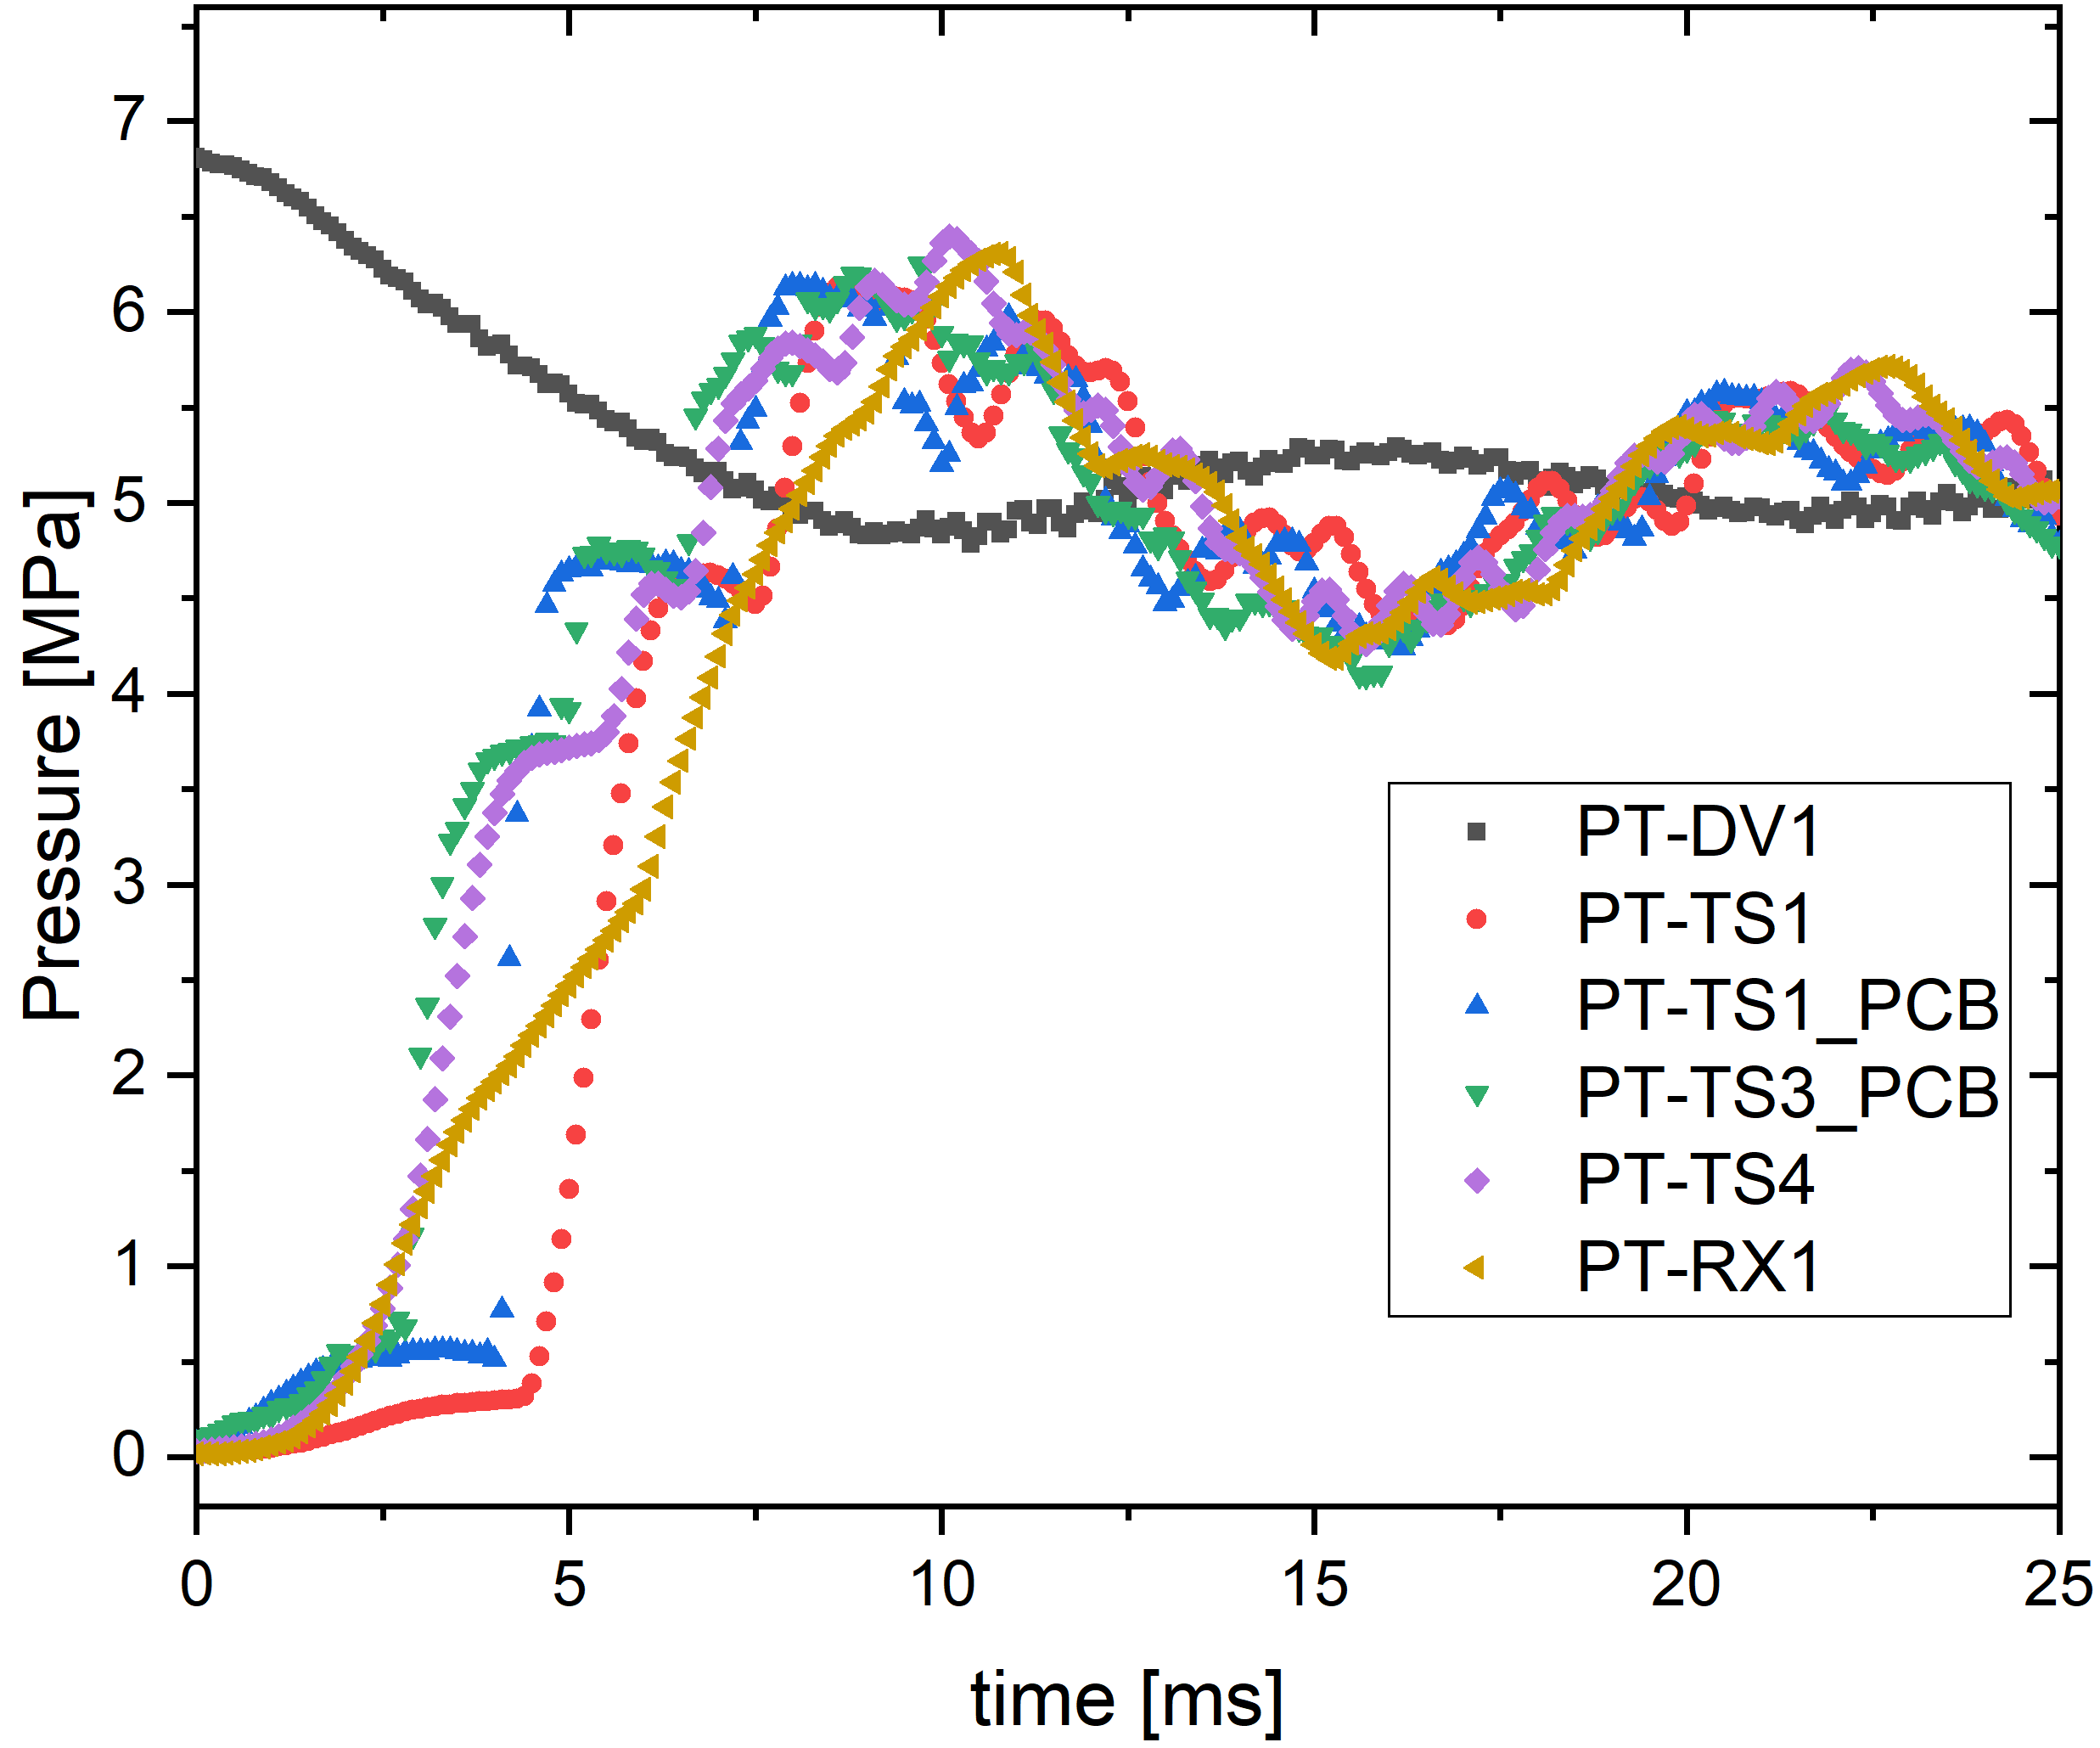
\includegraphics[width=0.9\textwidth]{results/plots/1000psi_Mpa_25.png}
        \caption{Pressure over time for a test using a FFKM o-ring on the second generation plug design.}
        \label{fig:piston 1000psi 25ms}
    \end{subfigure}
    
    \caption{Comparison of rupture disk and improved piston valve HENRI tests in a cylindrical test section at an initial pressure of \SI{6.9}{\mega\pascal} (\SI{1000}{psia}) and with intermediate tube inner diameter of \SI{2.54}{\centi\meter} (\SI{1}{inch}).}
    \label{fig:new piston v disk}
    \vspace{16pt}
\end{figure}

%%%%%%%%%%%%%%%%%%%%%%%%%%%%%%%%%%%%%%%%%%%%%%%%%%%%%%%%%%%%%%%%%%%%%%%%%%%%%%%%%%
% subsection about new piston valve repeatability
%\subsection{Improved Piston Valve Repeatability} \label{ss:new repeatability}



The repeatability is tested in the same manner as the first piston valve design. The piston valve is tested at the same initial pressure to determine the repeatability and consistency, then the valve is tested at varying initial pressures to provide data to predict the valve's operation and pressure evolution over a range of pressures. \Cref{fig:new piston 2 test} shows two tests at an initial pressure of \SI{6.9}{\mega\pascal} (1000 psi). The two tests overlap each other extremely well and demonstrate the improved piston valve can produce the same pressurization in the HENRI cartridge for multiple tests. \Cref{fig:new norm} presents tests over a range of initial pressures, normalized by the initial pressure. The highest three initial pressures provide very similar results, that also match well with the rupture disk tests. Tests with an initial pressure of \SI{2.5}{\mega\pascal} (360 psi) and lower, however, deviate from the trend of the other initial pressures. The characteristic pressure jumps associated with the shock wave are not as prominent, suggesting the valve is opening slower. The behavior of the valve and HENRI cartridge at low initial pressure is useful to know so TREAT has more flexibility in transient capability. The improved piston valve design also can seal at much lower pressures than the metal only plug design, which further increases the capability of the system.



\begin{figure}[bt]
    \centering
    \begin{subfigure}[t]{0.45\textwidth}
        \centering
        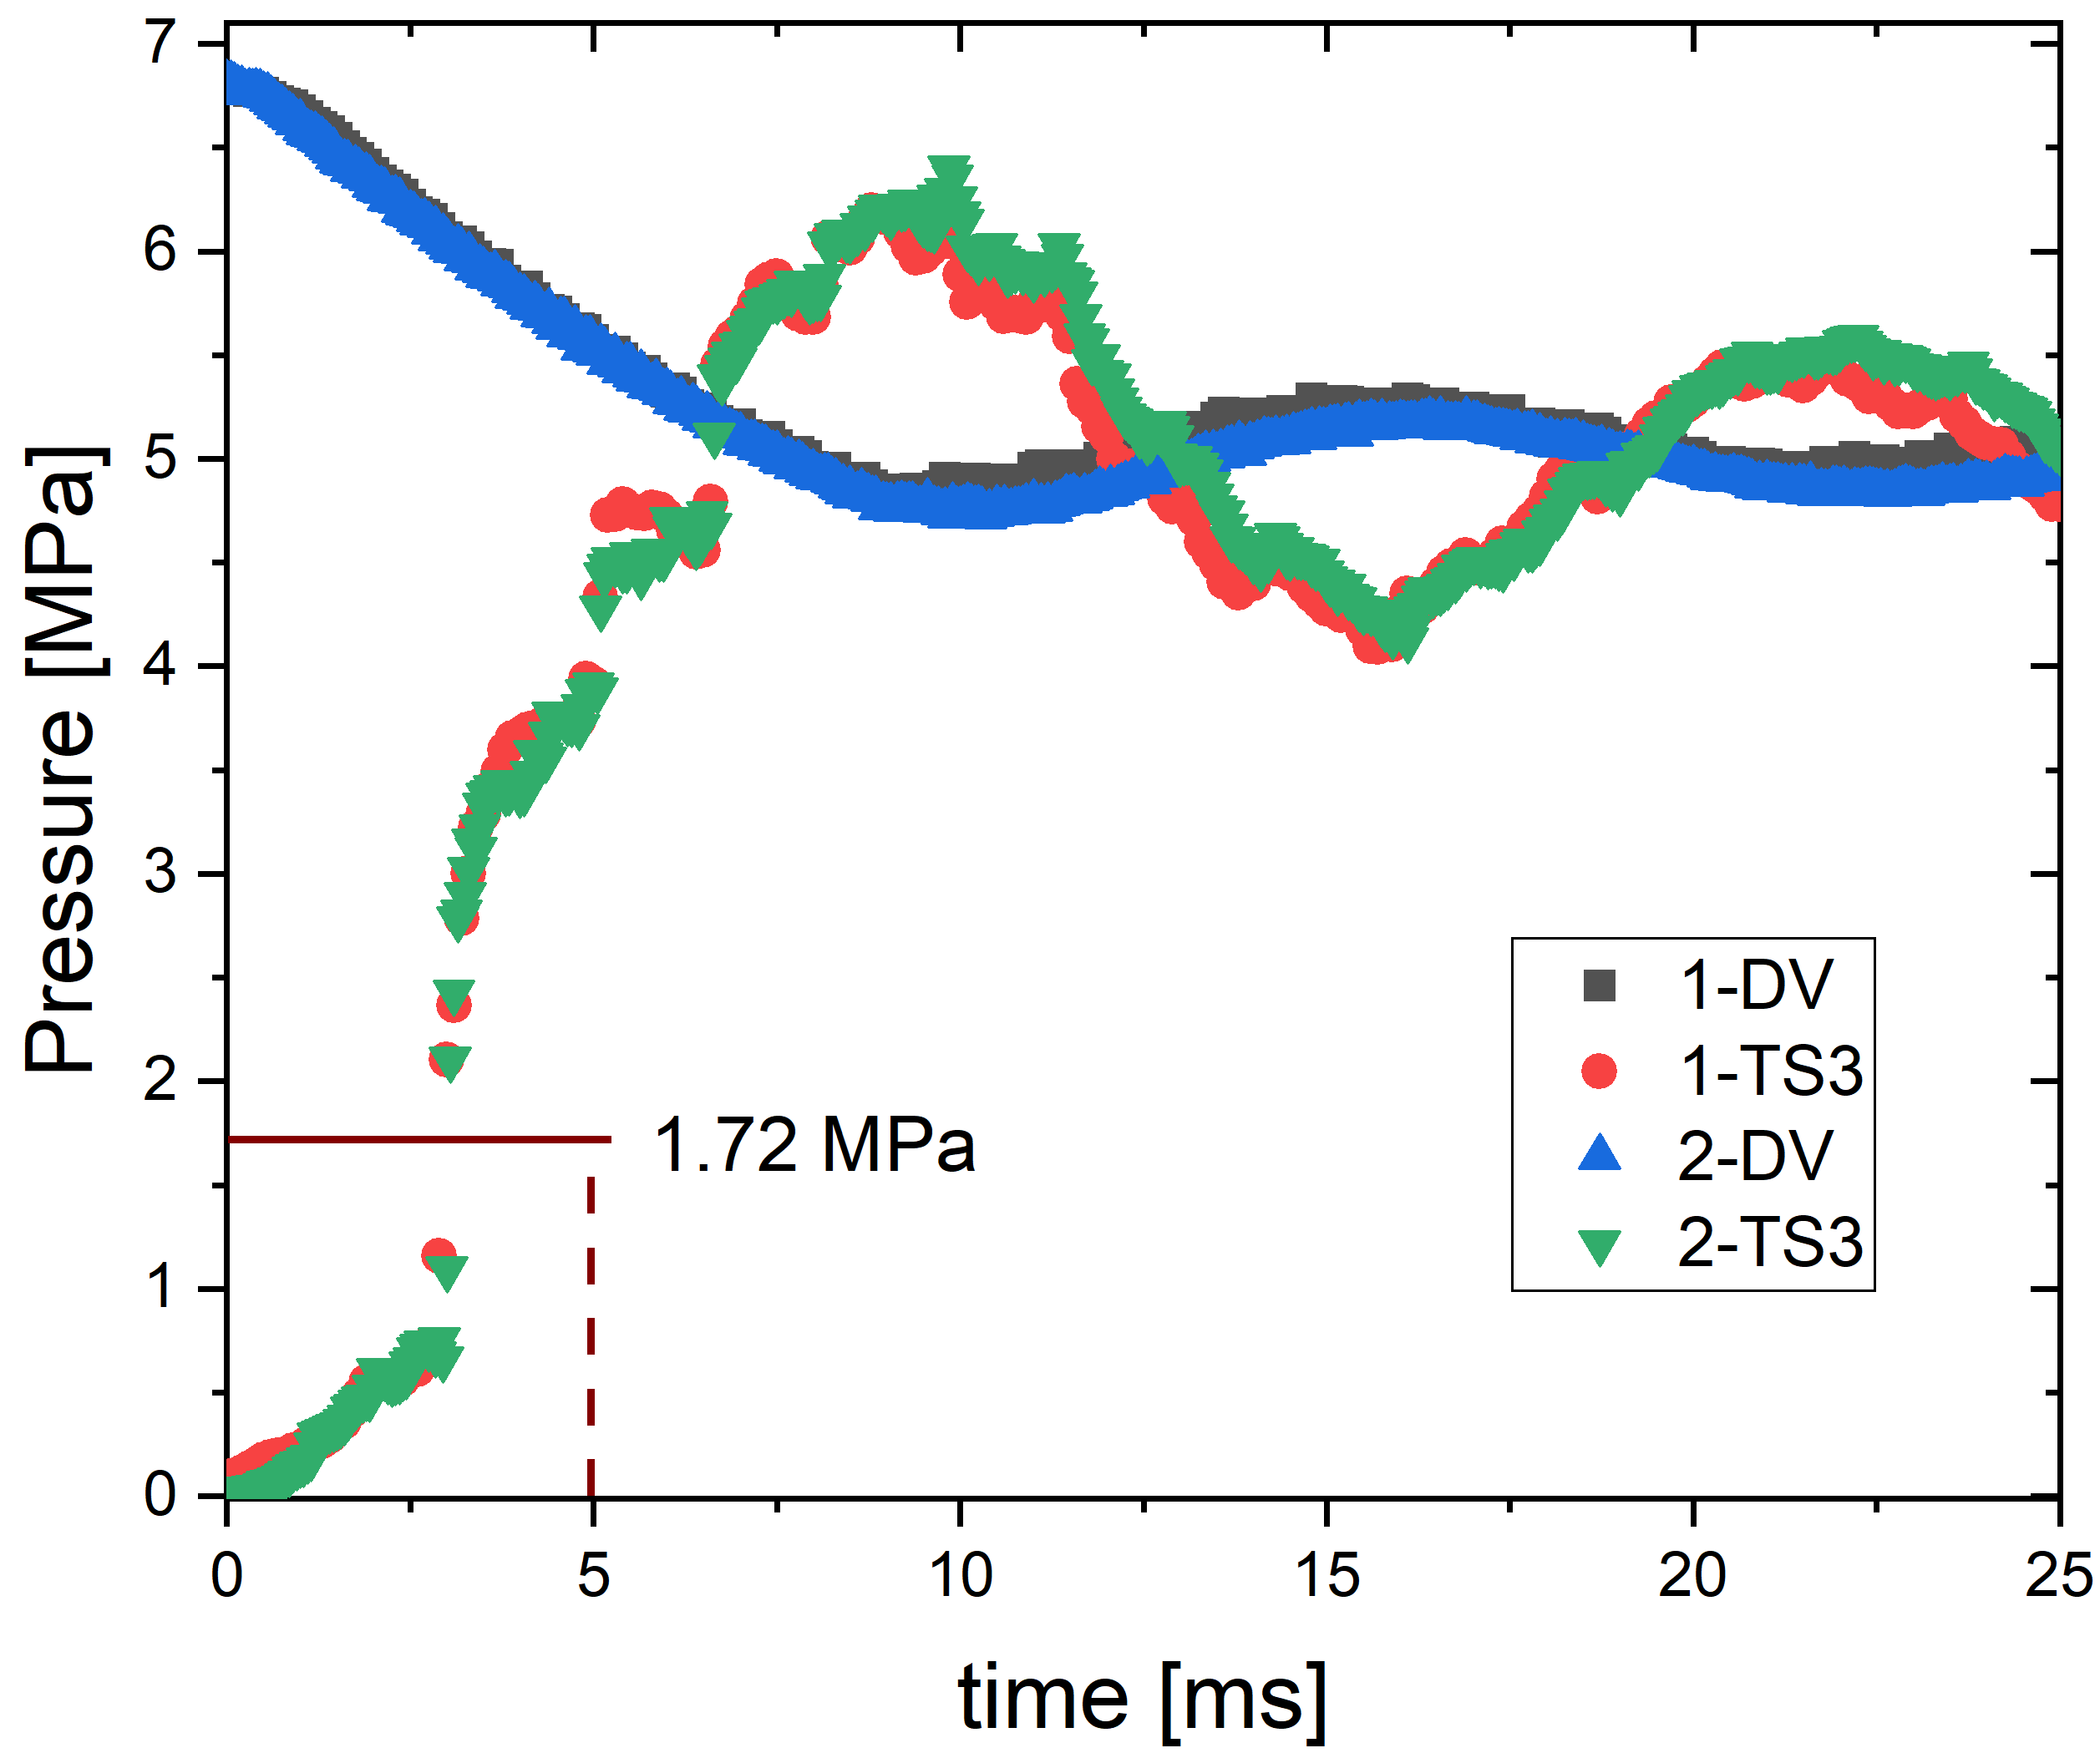
\includegraphics[width=0.9\textwidth]{results/plots/1000psi_FFKM_Piston_2.png}
        \caption{Comparison of two improved piston valve tests at an initial pressure of \SI{6.9}{\mega\pascal} (1000 psi).}
        \label{fig:new piston 2 test}
    \end{subfigure}
    \hfill
    \begin{subfigure}[t]{0.45\textwidth}
        \centering
        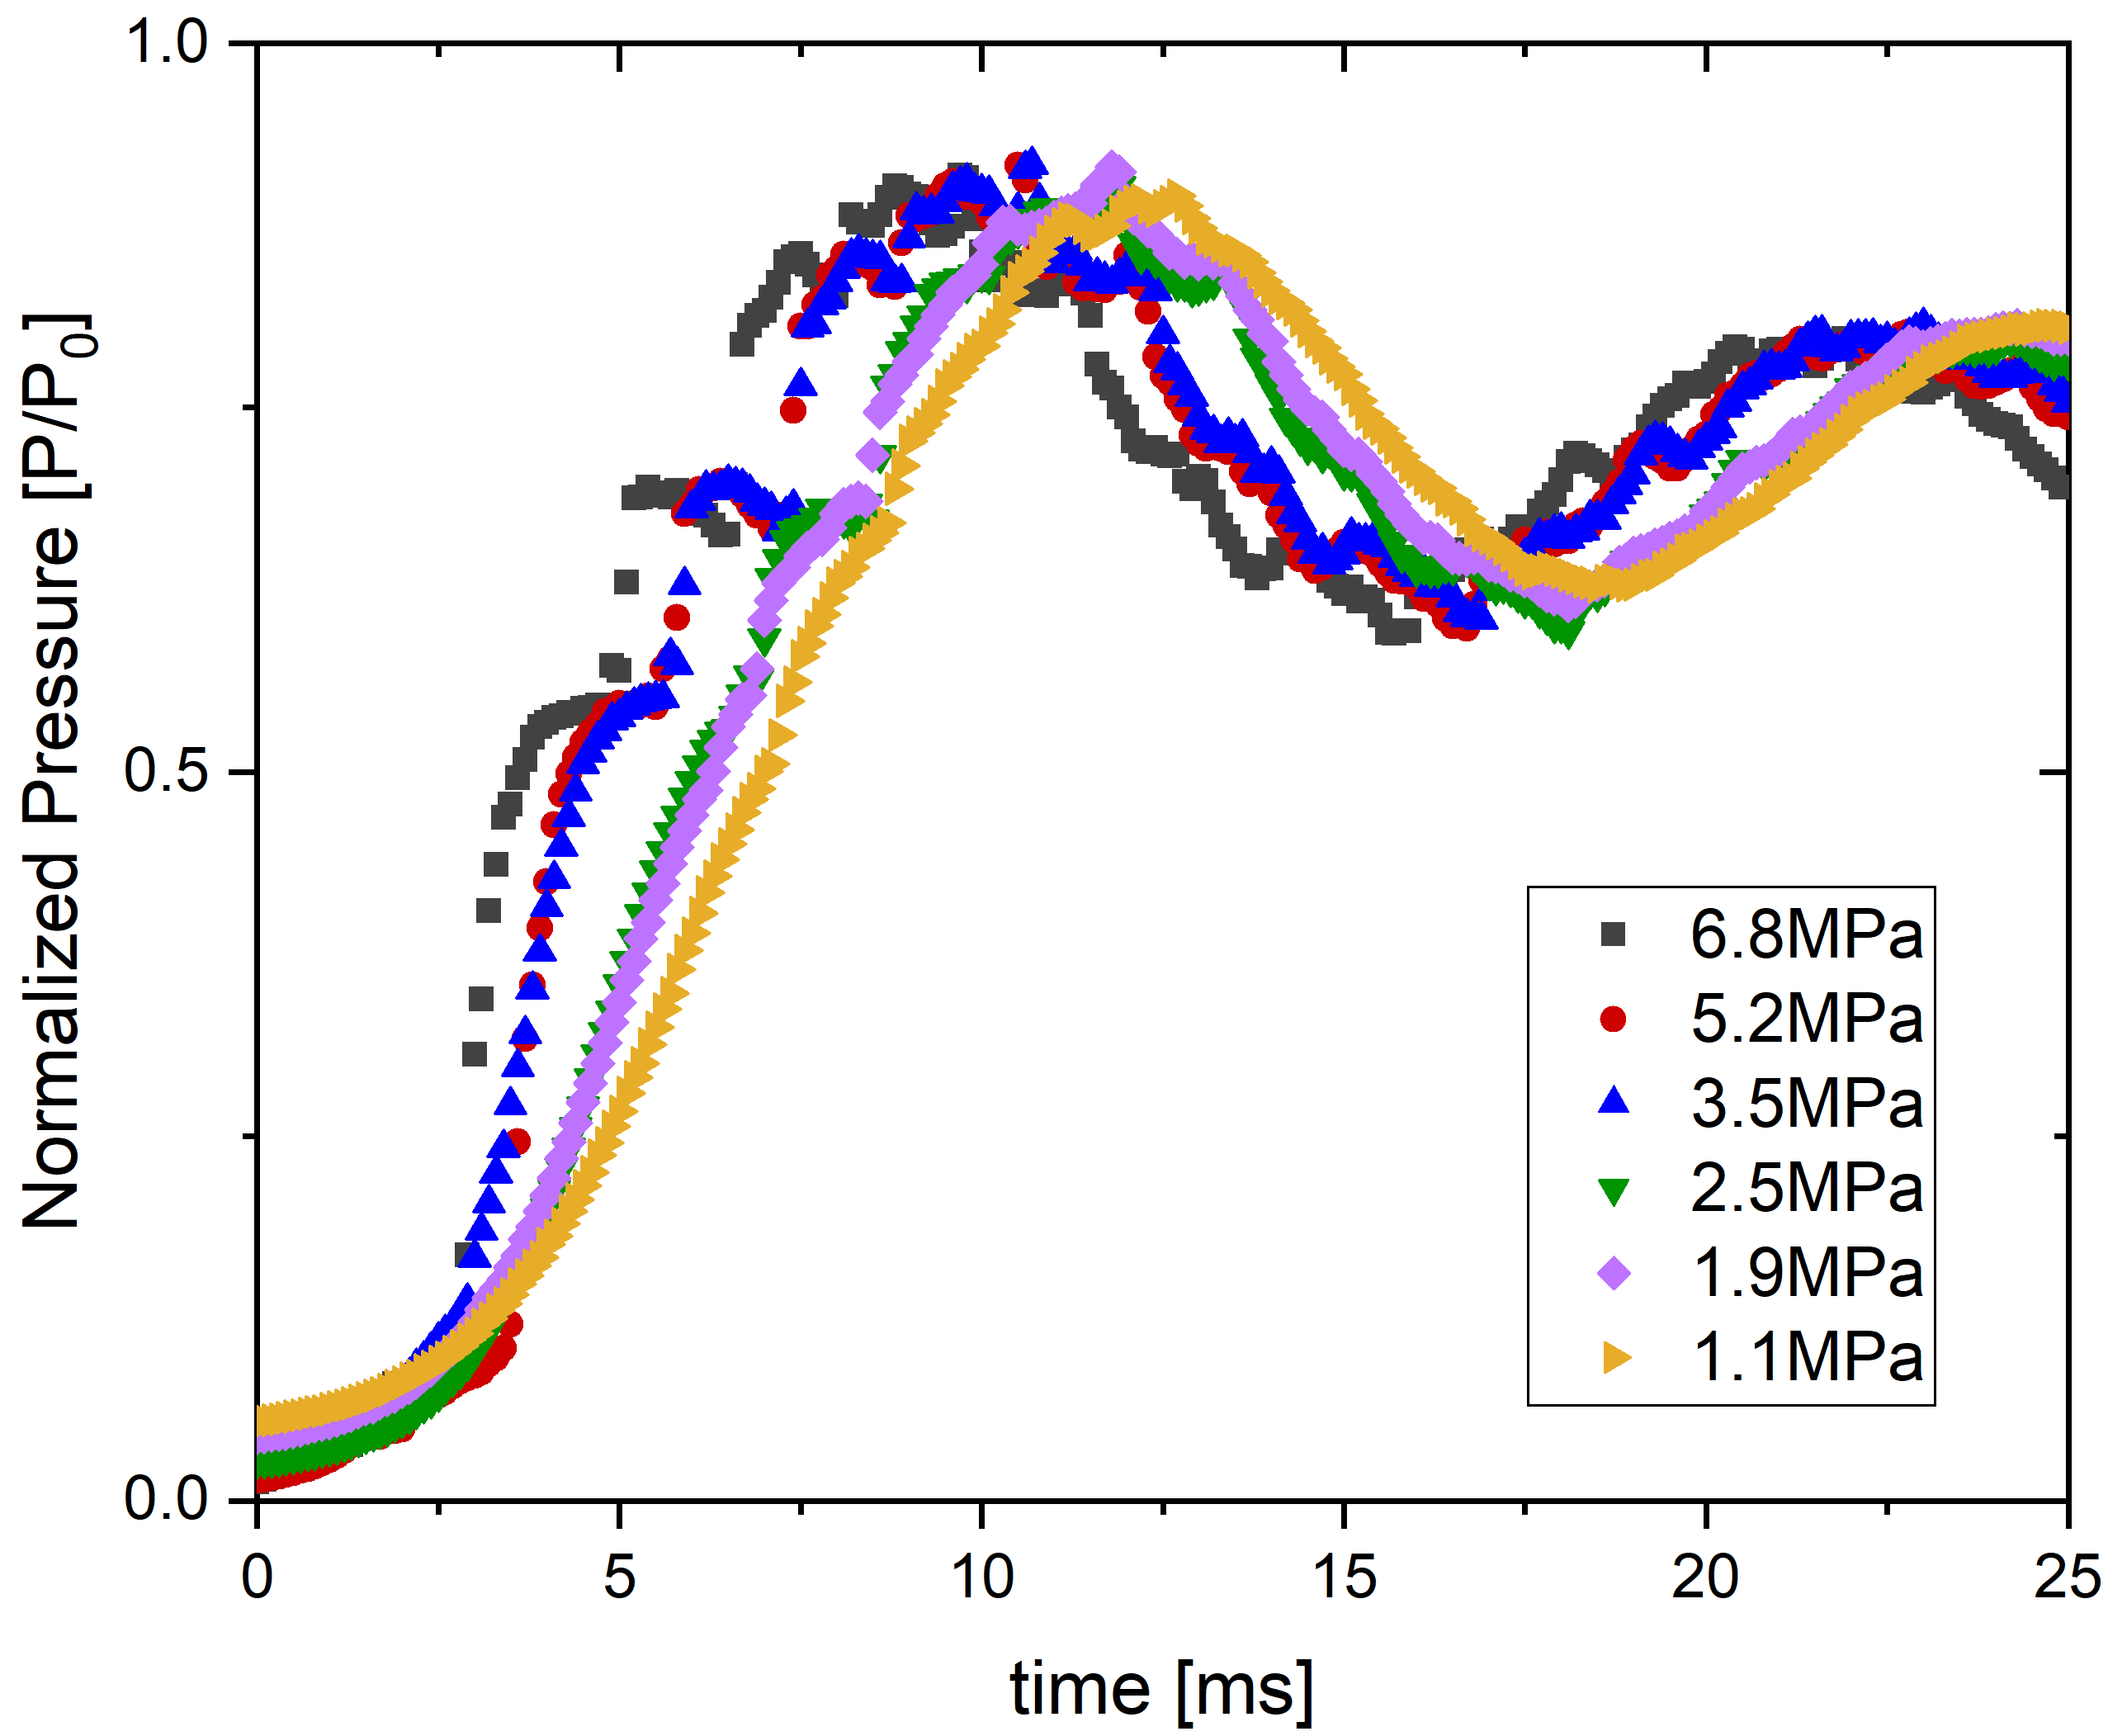
\includegraphics[width=0.9\textwidth]{results/plots/Normalized_TS3_oring.png}
        \caption{Improved piston valve test results, at position TS3, normalized by initial driver tank pressure for a range of initial driver tank pressures.}
        \label{fig:new norm}
    \end{subfigure}
    \caption{Comparison of results for improved piston valve to demonstrate repeatability at one initial pressure and predictability at varying initial pressures.}
    \label{fig:new piston repeatability}
\end{figure}







